\pdfinfoomitdate=1
\pdftrailerid{}
\pdfsuppressptexinfo=-1
\documentclass[10pt,a4paper]{article}
\usepackage{cmap}
\usepackage[margin=1.8cm,headheight=14pt,headsep=10pt]{geometry}
\usepackage[leqno]{amsmath}
\usepackage{amssymb,booktabs,longtable,array,ragged2e,multicol,multirow,xcolor,fancyhdr,tikz}
\definecolor{linkblue}{rgb}{0.08,0.33,0.58}
\usepackage[colorlinks=true,linkcolor=linkblue,urlcolor=linkblue,citecolor=linkblue,
  filecolor=linkblue,linktoc=all,pdfborder={0 0 0},bookmarksnumbered=true]{hyperref}
\setlength{\parindent}{0pt}\setlength{\parskip}{4pt}
\setcounter{secnumdepth}{2}\setcounter{tocdepth}{2}
\definecolor{partshade}{gray}{0.9}
\usepackage{nicefrac}
\definecolor{parttitle}{HTML}{295A2C}
\definecolor{parttitlelight}{HTML}{6C9F6D}
\makeatletter
\renewcommand\section{\@startsection{section}{1}{\z@}{-3ex plus -1ex minus -.2ex}%
  {1.2ex plus .2ex}{\normalfont\large\sffamily\bfseries\color{parttitle}}}
\renewcommand\subsection{\@startsection{subsection}{2}{\z@}{-2.5ex plus -1ex minus -.2ex}%
  {.8ex plus .2ex}{\normalfont\sffamily\bfseries\color{parttitle}}}
\renewcommand\subsubsection{\@startsection{subsubsection}{3}{\z@}{-2ex plus -1ex minus -.2ex}%
  {.6ex plus .2ex}{\normalfont\small\sffamily\bfseries\color{parttitle}}}
\renewcommand\paragraph{\@startsection{paragraph}{4}{\z@}{1.5ex plus .5ex minus .2ex}{-1em}%
  {\normalfont\small\sffamily\bfseries\color{parttitle}}}
\renewcommand\tagform@[1]{\maketag@@@{\textsf{\bfseries\footnotesize (#1)}}}
\renewcommand*\l@part[2]{\par\addvspace{1.6ex}\noindent{\sffamily\bfseries #1}\hfill
  {\sffamily\bfseries #2}\par\nobreak}
\newcommand\tocnumber{1.8em}
\newcommand\tocline[4]{\par{\rightskip \tocnumber plus 1fil\relax\parfillskip -\rightskip
  \noindent\hangindent\dimexpr#1+#2\relax\hspace*{#1}%
  \@tempdima #2{\sffamily\small #3}\nobreak\leaders\hbox{$\m@th\mkern 4.5mu\hbox{.}%
  \mkern 4.5mu$}\hfill\nobreak\hbox to \tocnumber{\hfil\sffamily\small #4}\par}}
\renewcommand*\l@section[2]{\tocline{0em}{2.2em}{#1}{#2}}
\renewcommand*\l@subsection[2]{\tocline{2.2em}{2.6em}{#1}{#2}}
\newcommand\contentspage{{\setlength{\columnsep}{24pt}\begin{multicols}{2}\@starttoc{toc}%
  \end{multicols}}}
\newcounter{docpart}\@addtoreset{section}{docpart}
\renewcommand\thesection{\ifnum\value{docpart}>0 \arabic{docpart}.\fi\arabic{section}}
\renewcommand\theHsection{\arabic{docpart}.\arabic{section}}
\newcommand\partnumber[1]{#1\enspace}
\pdfstringdefDisableCommands{\def\partnumber#1{#1 }}
\newcommand{\partbox}[1]{\par\addvspace{12pt}\refstepcounter{docpart}\phantomsection
  \addcontentsline{toc}{part}{\protect\partnumber{\thedocpart}#1}%
  \noindent\colorbox{partshade}{\makebox[%
  \dimexpr\textwidth-2\fboxsep\relax]{\rule[-6pt]{0pt}{20pt}\Large\sffamily\bfseries%
  \textcolor{parttitle}{\thedocpart\quad #1}}}\par\nobreak\@nobreaktrue\addvspace{2pt}}
\newmarks\LTstartmarks\newcount\LTstartcount
\let\LT@startplain\LT@start
\def\LT@start{\global\advance\LTstartcount\@ne\LT@startplain
  \marks\LTstartmarks{\the\LTstartcount}}
\newmarks\LTgroupmarks
\newcount\LTspacebreak\LTspacebreak=-1
\newcount\LTrulebreak\LTrulebreak=-2
\def\grouprule#1#2{\noalign{\marks\LTgroupmarks{\the\belowrulesep}\nobreak\vskip#1%
  \vskip\aboverulesep}\multispan\LT@cols\unskip{\leaders\hrule\@height#2\hfill\kern\z@}\cr
  \noalign{\penalty\LTrulebreak\vskip\belowrulesep\global\@lastruleclass\z@}}
\def\groupspace#1{\noalign{\marks\LTgroupmarks{\the\dimexpr#1\relax}\penalty\LTspacebreak
  \vskip#1\global\@lastruleclass\z@}}
\def\LT@unskips{\unskip\unpenalty\unskip\unpenalty\unskip\unpenalty\unskip\unpenalty}
\def\LT@groupcut{\ifnum\outputpenalty=\LTrulebreak
  \setbox\@cclv\vbox{\unvbox\@cclv\setbox\z@\lastbox\LT@unskips}\fi}
\def\LT@groupjoin{\ifnum\outputpenalty=\LTspacebreak\vskip-\botmarks\LTgroupmarks\relax\fi
  \ifnum\outputpenalty=\LTrulebreak\vskip-\botmarks\LTgroupmarks\relax\fi}
\let\LT@outputplain\LT@output
\def\LT@output{\ifnum\outputpenalty<-\@Mi\LT@outputplain\else
  \edef\LT@marka{\botmarks\LTstartmarks}\edef\LT@markb{\the\LTstartcount}%
  \ifx\LT@marka\LT@markb\LT@groupcut\LT@outputplain\LT@groupjoin
  \else\setbox\LT@head\box\voidb@x\LT@outputplain\fi\fi}
\makeatother
\newcommand{\needspace}[1]{\par\penalty-100\begingroup\dimen0=#1\relax\dimen2=\pagegoal
  \advance\dimen2-\pagetotal\ifdim\dimen0>\dimen2\relax\ifdim\dimen2>0pt\vfil\break\fi\fi
  \endgroup}
\numberwithin{equation}{section}
\pagestyle{fancy}\fancyhf{}
\renewcommand{\headrulewidth}{0pt}
\renewcommand{\sectionmark}[1]{\markright{\thesection\enspace #1}}
\renewcommand{\subsectionmark}[1]{}
\fancyhead[R]{\small\textsc{\rightmark}\quad\thepage}
\fancypagestyle{plain}{\fancyhf{}\fancyfoot[C]{\small\thepage}}
\definecolor{atlasI}{HTML}{991A1A}\definecolor{atlasIl}{HTML}{EC6B60}
\definecolor{atlasII}{HTML}{295A2C}\definecolor{atlasIIl}{HTML}{6C9F6D}
\definecolor{atlasIII}{HTML}{7A1466}\definecolor{atlasIIIl}{HTML}{D66EBC}
\definecolor{atlasIV}{HTML}{9B690B}\definecolor{atlasIVl}{HTML}{F2A618}
\makeatletter
\newcommand\atlas@full{%
\fill[atlasIII] (0.0394,0.0163) -- (0.3978,0.0163) arc[start angle=0.668, end angle=13.836, radius=1.3979] -- cycle;
\fill[atlasI] (-0.0163,0.0394) -- (-0.0163,0.3978) arc[start angle=90.668, end angle=103.836, radius=1.3979] -- cycle;
\fill[atlasIV] (-0.0394,-0.0163) -- (-0.3978,-0.0163) arc[start angle=-179.332, end angle=-166.164, radius=1.3979] -- cycle;
\fill[atlasII] (0.0163,-0.0394) -- (0.0163,-0.3978) arc[start angle=-89.332, end angle=-76.164, radius=1.3979] -- cycle;
\fill[atlasIIIl] (0.0163,0.0394) -- (0.3343,0.3573) arc[start angle=76.164, end angle=89.332, radius=1.3979] -- cycle;
\fill[atlasIl] (-0.0394,0.0163) -- (-0.3573,0.3343) arc[start angle=166.164, end angle=179.332, radius=1.3979] -- cycle;
\fill[atlasIVl] (-0.0163,-0.0394) -- (-0.3343,-0.3573) arc[start angle=-103.836, end angle=-90.668, radius=1.3979] -- cycle;
\fill[atlasIIl] (0.0394,-0.0163) -- (0.3573,-0.3343) arc[start angle=-13.836, end angle=-0.668, radius=1.3979] -- cycle;
\fill[atlasIIIl] (0.4304,0.0163) -- (0.9598,0.0163) arc[start angle=46.637, end angle=73.849, radius=1.3979] arc[start angle=13.862, end angle=0.653, radius=1.4305] -- cycle;
\fill[atlasIl] (-0.0163,0.4304) -- (-0.0163,0.9598) arc[start angle=136.637, end angle=163.849, radius=1.3979] arc[start angle=103.862, end angle=90.653, radius=1.4305] -- cycle;
\fill[atlasIVl] (-0.4304,-0.0163) -- (-0.9598,-0.0163) arc[start angle=-133.363, end angle=-106.151, radius=1.3979] arc[start angle=-166.138, end angle=-179.347, radius=1.4305] -- cycle;
\fill[atlasIIl] (0.0163,-0.4304) -- (0.0163,-0.9598) arc[start angle=-43.363, end angle=-16.151, radius=1.3979] arc[start angle=-76.138, end angle=-89.347, radius=1.4305] -- cycle;
\fill[atlasIII] (0.0163,0.4304) arc[start angle=89.347, end angle=76.138, radius=1.4305] arc[start angle=16.151, end angle=43.363, radius=1.3979] -- cycle;
\fill[atlasI] (-0.4304,0.0163) arc[start angle=179.347, end angle=166.138, radius=1.4305] arc[start angle=106.151, end angle=133.363, radius=1.3979] -- cycle;
\fill[atlasIV] (-0.0163,-0.4304) arc[start angle=-90.653, end angle=-103.862, radius=1.4305] arc[start angle=-163.849, end angle=-136.637, radius=1.3979] -- cycle;
\fill[atlasII] (0.4304,-0.0163) arc[start angle=-0.653, end angle=-13.862, radius=1.4305] arc[start angle=-73.849, end angle=-46.637, radius=1.3979] -- cycle;
\fill[atlasIII] (0.9997,0.0232) arc[start angle=1.329, end angle=44.066, radius=1] -- (0.3973,0.3742) arc[start angle=73.875, end angle=45.664, radius=1.4305] -- cycle;
\fill[atlasI] (-0.0232,0.9997) arc[start angle=91.329, end angle=134.066, radius=1] -- (-0.3742,0.3973) arc[start angle=163.875, end angle=135.664, radius=1.4305] -- cycle;
\fill[atlasIV] (-0.9997,-0.0232) arc[start angle=-178.671, end angle=-135.934, radius=1] -- (-0.3973,-0.3742) arc[start angle=-106.125, end angle=-134.336, radius=1.4305] -- cycle;
\fill[atlasII] (0.0232,-0.9997) arc[start angle=-88.671, end angle=-45.934, radius=1] -- (0.3742,-0.3973) arc[start angle=-16.125, end angle=-44.336, radius=1.4305] -- cycle;
\fill[atlasIIIl] (0.0232,0.9997) arc[start angle=44.336, end angle=16.125, radius=1.4305] -- (0.6955,0.7185) arc[start angle=45.934, end angle=88.671, radius=1] -- cycle;
\fill[atlasIl] (-0.9997,0.0232) arc[start angle=134.336, end angle=106.125, radius=1.4305] -- (-0.7185,0.6955) arc[start angle=135.934, end angle=178.671, radius=1] -- cycle;
\fill[atlasIVl] (-0.0232,-0.9997) arc[start angle=-135.664, end angle=-163.875, radius=1.4305] -- (-0.6955,-0.7185) arc[start angle=-134.066, end angle=-91.329, radius=1] -- cycle;
\fill[atlasIIl] (0.9997,-0.0232) arc[start angle=-45.664, end angle=-73.875, radius=1.4305] -- (0.7185,-0.6955) arc[start angle=-44.066, end angle=-1.329, radius=1] -- cycle;
}
\newcommand\atlas@draw[2]{\begin{tikzpicture}[x=\dimexpr(#1)/2\relax,y=\dimexpr(#1)/2\relax]
\useasboundingbox (-1,-1) rectangle (1,1);#2\end{tikzpicture}}
\newcommand\atlas@volume[1]{{%
\colorlet{atlasI}{parttitle}\colorlet{atlasIl}{parttitlelight}%
\colorlet{atlasII}{parttitle}\colorlet{atlasIIl}{parttitlelight}%
\colorlet{atlasIII}{parttitle}\colorlet{atlasIIIl}{parttitlelight}%
\colorlet{atlasIV}{parttitle}\colorlet{atlasIVl}{parttitlelight}%
#1}}
\newcommand\atlasmark[1]{\atlas@draw{#1}{\atlas@full}}
\newcommand\volumemark[1]{\atlas@volume{\atlasmark{#1}}}
\makeatother
\fancypagestyle{opening}{\fancyhf{}\fancyfoot[C]{\small\thepage}%
  \fancyhead[L]{\smash{\raisebox{-9.5mm}{\volumemark{12mm}}}}}
\hypersetup{pdftitle={Pinminus3: Point Group Atlas, volume II: double point groups}, pdfsubject={Point Group Atlas double record Pinminus3, schema point-group-atlas/double/group-continuous/1}}
\fancyhead[L]{\small $\grp{Pin^{-}(3)}$}
\DeclareMathAlphabet{\mathelt}{OT1}{cmss}{m}{sl}
\DeclareSymbolFont{eltgreek}{OML}{cmssm}{m}{it}
\DeclareMathSymbol{\eltsigma}{\mathord}{eltgreek}{"1B}
\DeclareSymbolFont{eltletters}{OT1}{cmss}{m}{sl}
\DeclareMathSymbol{g}{\mathalpha}{eltletters}{`g}
\DeclareMathSymbol{h}{\mathalpha}{eltletters}{`h}
\DeclareMathSymbol{Q}{\mathalpha}{eltletters}{`Q}
\DeclareMathSymbol{R}{\mathalpha}{eltletters}{`R}
\DeclareMathSymbol{\xi}{\mathord}{eltgreek}{"18}
\newcommand{\eltfont}[1]{{\let\sigma\eltsigma\mathelt{#1}}}
\newcommand{\grp}[1]{\mathsf{#1}}
\newcommand{\irr}[1]{\text{\normalfont\scshape #1}}
\newcommand{\conjpair}[1]{{}^{#1}}
\newcommand{\detbox}[1]{{\setlength{\fboxsep}{1pt}\fbox{#1}}}
\newcommand{\cls}[1]{\eltfont{#1}}
\newcommand{\comp}[1]{\eltfont{#1}}
\newcommand{\elt}[1]{\eltfont{#1}}
\newcommand{\hmname}[1]{#1}
\newcommand{\conwayname}[1]{#1}
\newcommand{\ptag}[1]{\mathrm{#1}}
\newcommand{\orbital}[1]{\mathrm{#1}}
\newcommand{\dirprod}{\times}
\newcommand{\sdprod}{\rtimes}
\newcommand{\samecls}{\cong}
\newcommand{\nconj}[1]{{\scriptsize$\times#1$}}
\newcommand{\clsletter}[1]{\,{\scriptsize\color{black!55}#1}}
\newcommand{\metclasses}[1]{\,{\scriptsize$\{#1\}$}}
\newcommand{\Cyc}[1]{\grp{Z_{#1}}}
\newcommand{\Sym}[1]{\grp{Sym_{#1}}}
\newcommand{\dirvec}[3]{(#1, #2, #3)}
\newcommand{\grpindex}[2]{[#1 : #2]}
\newcommand{\iverson}[1]{[#1]}
\newcommand{\restr}[2]{#1\!\downarrow#2}
\newcommand{\Ind}[2]{\operatorname{Ind}_{#1}^{#2}}
\newcommand{\genidx}[2]{#1^{[\mathrm{#2}]}}
\newcommand{\pointr}{\mathbf{r}}
\newcommand{\unitaxis}{\hat{\mathbf{v}}}
\newcommand{\vv}{\mathbf{v}}
\newcommand{\iunit}{\mathrm{i}}
\newcommand{\expe}{\mathrm{e}}
\newcommand{\diff}{\mathrm{d}}
\newcommand{\goldenratio}{\varphi}
\newcommand{\rootunity}[1]{\zeta_{#1}}
\newcommand{\irrJ}[1]{D^{(#1)}}
\newcommand{\irrJp}[2]{D^{(#1,#2)}}
\newcommand{\repD}[1]{D^{#1}}
\newcommand{\wignerD}[1]{D^{#1}}
\newcommand{\wignerd}[1]{d^{#1}}
\newcommand{\irchar}[1]{\chi_{#1}}
\newcommand{\chiA}{\chi_{\grp{A}}}
\newcommand{\fsind}{\nu_{\mathrm{FS}}}
\newcommand{\conj}[1]{{#1}^{*}}
\newcommand{\diag}{\operatorname{diag}}
\newcommand{\trace}{\operatorname{tr}}
\newcommand{\irrprod}{\otimes}
\newcommand{\mult}{\kappa}
\newcommand{\intx}{\mu}
\newcommand{\cgnorm}{\mathcal{N}}
\newcommand{\period}{L}
\newcommand{\jm}[2]{\bigl\lvert{}^{#1}_{\,#2}\bigr\rangle}
\newcommand{\cgket}[3]{\bigl\lvert{}^{#1}_{\,#2};#3\bigr\rangle}
\newcommand{\irket}[2]{\bigl\lvert{}^{#1}_{\,#2}\bigr\rangle}
\newcommand{\prodket}[2]{\lvert {#1}\,{#2}\rangle}
\newcommand{\ket}[1]{\lvert #1\rangle}
\newcommand{\cgc}[6]{\bigl\langle{}^{#1}_{\,#2}\,{}^{#3}_{\,#4}\bigm\vert{}^{#5}_{\,#6}\bigr\rangle}
\newcommand{\cgck}[7]{\bigl\langle{}^{#1}_{\,#2}\,{}^{#3}_{\,#4}\bigm\vert{}^{#5}_{\,#6};#7\bigr\rangle}
\newcommand{\cgcone}[3]{\langle #1\,#2\mid #3\rangle}
\newcommand{\irrangle}{\text{--}}
\newcommand{\vol}{\operatorname{vol}}
\newcommand{\fcell}{\mathcal{D}}
\newcommand{\fdomain}{\mathcal{F}}
\newcommand{\lensspace}[2]{\mathsf{L}(#1, #2)}
\newcommand{\twosphere}{\mathsf{S}^{2}}
\newcommand{\projplane}{\mathbb{R}\mathsf{P}^{2}}
\newcommand{\term}[2]{{}^{#1}#2}
\newcommand{\barred}[1]{\bar{#1}}
\newcommand{\Quat}[1]{\grp{Q_{#1}}}
\newcommand{\SL}[1]{\grp{SL}(2,#1)}
\newcommand{\secondclass}{\mathrm{b}}
\newcommand{\dmark}{{}^{d}}
\newcommand{\lift}[1]{\tilde{#1}}
\newcommand{\pauli}[1]{\sigma_{#1}}
\newcommand{\paulivec}{\vec{\sigma}}
\newcommand{\hairsp}{\mkern1mu}
\newenvironment{romanlist}{\begin{enumerate}%
\renewcommand{\labelenumi}{(\roman{enumi})}}%
  {\end{enumerate}}
\makeatletter
\newenvironment{irmatrix}[1]{\null\,\vcenter\bgroup\Let@\restore@math@cr\default@tag
  \baselineskip8\ex@ \lineskip3\ex@ \lineskiplimit\lineskip
  \ialign\bgroup\hfil$\m@th\scriptstyle##$\hfil&&\hskip#1\hfil$\m@th\scriptstyle##$\hfil\crcr}%
  {\crcr\egroup\egroup\,}
\makeatother
\newlength{\fillwidth}\newlength{\cellwidth}\newlength{\colwidth}
\newcommand{\cellmax}[1]{\settowidth{\cellwidth}{#1}%
  \ifdim\cellwidth>\colwidth\setlength{\colwidth}{\cellwidth}\fi}
\newcommand{\fillcap}{\ifdim\colwidth<\fillwidth\setlength{\fillwidth}{\colwidth}\fi}
\newcommand{\signbreak}{\penalty100\relax}
\begin{document}
\thispagestyle{opening}
\begin{center}
{\LARGE\sffamily\bfseries\color{parttitle}The group $\grp{Pin^{-}(3)}$}
\end{center}
\contentspage
\needspace{194pt}
\partbox{The group}
\section{Names and structure}\label{s:identification}
Conventions: \href{../../CONVENTIONS.pdf}{CONVENTIONS.pdf}, sections \href{../../../rotation/CONVENTIONS.pdf\#conv.0.1}{0.1}, \href{../../../rotation/CONVENTIONS.pdf\#conv.2}{2}, \href{../../../rotation/CONVENTIONS.pdf\#conv.12}{12}, \href{../../CONVENTIONS.pdf\#conv.20}{20} and \href{../../CONVENTIONS.pdf\#conv.29}{29}.
\label{n:mark.classes}{\small\begin{longtable}{@{}ll@{}}\toprule
\texttt{symbol} & \href{Pinminus3.pdf}{$\grp{Pin^{-}(3)}$}\\
\texttt{cover\symbol{95}of} & \href{../../../rotation/data/pdf/O3.pdf}{$\grp{O(3)}$}\\
\grouprule{0pt}{\lightrulewidth}
\texttt{abstract\symbol{95}type} & $\grp{SU(2)}\dirprod \Cyc{2}$\\
\grouprule{0pt}{\lightrulewidth}
\texttt{su2\symbol{95}subgroup} & \href{SU2.pdf}{$\grp{SU(2)}$}, index 2\\
\texttt{normalizer} & \href{Pinminus3.pdf}{$\grp{Pin^{-}(3)}$}, index 1\\
\texttt{centralizer} & \href{2S2.pdf}{$\grp{2C_{i}}$}\\
\texttt{product\symbol{95}form} & \begin{tabular}[t]{@{}l@{}}direct: \href{SU2.pdf}{$\grp{SU(2)}$}${}\dirprod{}$\href{S2.pdf}{$\grp{C_{i}}$}\metclasses{\cls{E}, \cls{\lift{i}}}; \href{SU2.pdf}{$\grp{SU(2)}$}${}\dirprod{}$\href{S2b.pdf}{$\grp{C_{i}}\secondclass$}\metclasses{\cls{E}, \cls{\barred{\lift{i}}}}\end{tabular}\\
\texttt{center} & \href{2S2.pdf}{$\grp{2C_{i}}$}\\
\texttt{commutator\symbol{95}subgroup} & \href{SU2.pdf}{$\grp{SU(2)}$}, index 2\\
\grouprule{0pt}{\lightrulewidth}
\texttt{alternative\symbol{95}names} & \href{Pinminus3.pdf}{$\grp{2K_{h}}$}\\
\texttt{hermann\symbol{95}mauguin} & $\dmark\hmname{\infty \infty m}$\\
\bottomrule\end{longtable}}
\leavevmode\label{n:group.preimage}The group $\grp{Pin^{-}(3)}$ is the double cover of \href{../../../rotation/data/pdf/O3.pdf}{$\grp{O(3)}$}, whose document sets the fields that this table does not repeat (\texttt{cover\symbol{95}of}): its type, geometry, crystal classes and the names of its \href{../../../rotation/data/pdf/O3.pdf}{$\grp{O(3)}$}-conjugacy class. This preimage is continuous, so its order and GAP identifier are undefined. The field \texttt{su2\symbol{95}subgroup} is $\grp{Pin^{-}(3)} \cap \grp{SU(2)}$, the largest subgroup of $\grp{Pin^{-}(3)}$ in $\grp{SU(2)}$ (its elements of parity $+1$), and \texttt{normalizer} and \texttt{centralizer} are taken in $\grp{Pin^{-}(3)}$.
In \texttt{product\symbol{95}form}, the braces contain the classes of $\grp{Pin^{-}(3)}$ that the finite second factor meets: atoms of the class space (section~\ref{s:class_space}) and distinguished points of its arcs (\href{../../CONVENTIONS.pdf}{CONVENTIONS.pdf}, sections \href{../../../rotation/CONVENTIONS.pdf\#conv.16}{16}, \href{../../CONVENTIONS.pdf\#conv.21}{21} and \href{../../CONVENTIONS.pdf\#conv.29.1}{29.1}).
\needspace{103pt}
\section{Class space}\label{s:class_space}
Conventions: \href{../../CONVENTIONS.pdf}{CONVENTIONS.pdf}, sections \href{../../../rotation/CONVENTIONS.pdf\#conv.16}{16}, \href{../../CONVENTIONS.pdf\#conv.21}{21} and \href{../../CONVENTIONS.pdf\#conv.29.1}{29.1}.
\leavevmode\label{n:head.component}A row is a component of the class space of $\grp{Pin^{-}(3)}$, an arc of classes. \label{n:head.coset}\label{n:head.element}A row gives whether its elements cover proper or improper elements of \href{../../../rotation/data/pdf/O3.pdf}{$\grp{O(3)}$} (coset) and the element of $\grp{Pin^{-}(3)}$ at its angle. \label{n:angle.omega}The elements at the angles are the lift $\lift{R}_z(\omega) = \cos\tfrac{\omega}{2} - \iunit\sin\tfrac{\omega}{2}\,\pauli{z}$, $0 \le \omega < 4\pi$, and its products $\elt{\lift{i}}\,\lift{R}_z(\omega)$ with the lift of the inversion $\elt{\lift{i}}$ (\href{../../CONVENTIONS.pdf}{CONVENTIONS.pdf}, section \href{../../CONVENTIONS.pdf\#conv.29.1}{29.1}). \label{n:matrix.element.pin}The matrix $M(g)$ of the element is the transpose of its $\grp{SU(2)}$ part, so that the matrices compose as the matrices $P(g)$ of the elements of \href{../../../rotation/data/pdf/O3.pdf}{$\grp{O(3)}$} (\href{../../CONVENTIONS.pdf}{CONVENTIONS.pdf}, section \href{../../CONVENTIONS.pdf\#conv.21.2}{21.2}).
The constant $\iunit$ is the imaginary unit, and $\expe$ is the base of the natural logarithm.
\begin{center}\begin{tabular}{@{}llll@{}}\toprule
component & coset & element & $M(g)$\\\midrule
$\comp{\lift{C}(\omega)}$ & proper & $\elt{\lift{C}}(\omega)$ & $\left(\begin{smallmatrix}\expe^{-\iunit\omega/2} & 0\\ 0 & \expe^{\iunit\omega/2}\end{smallmatrix}\right)$\\\addlinespace[6pt]
$\comp{\lift{i}\,\lift{C}(\omega)}$ & improper & $\elt{\lift{i}\,\lift{C}}(\omega)$ & $\left(\begin{smallmatrix}\expe^{-\iunit\omega/2} & 0\\ 0 & \expe^{\iunit\omega/2}\end{smallmatrix}\right)$\\
\bottomrule\end{tabular}\end{center}
On an arc, $\elt{\lift{R}_z}(\omega)$ is conjugate to $\elt{\lift{R}_z}(4\pi - \omega)$, so the classes run over $0 \le \omega \le 2\pi$, from $\cls{E}$ through the half turns to $\cls{\barred{E}}$.
The distinguished points are $\cls{E}$ at $\omega = 0$, $\cls{C_2}$ at $\omega = \pi$, $\cls{\barred{E}}$ at $\omega = 2\pi$, $\cls{\lift{i}}$ at $\omega = 0$, $\cls{\sigma_h}$ at $\omega = \pi$ and $\cls{\barred{\lift{i}}}$ at $\omega = 2\pi$.
\leavevmode\label{n:local.haar.h}The Haar measure, of total mass 1, is $\diff h = (1 - \cos\omega)\,\diff\omega/(4\pi)$ on $\comp{\lift{C}(\omega)}$, $\omega\in\bigl[0, 2\pi\bigr]$, of mass $\tfrac{1}{2}$, and $\diff h = (1 - \cos\omega)\,\diff\omega/(4\pi)$ on $\comp{\lift{i}\,\lift{C}(\omega)}$, $\omega\in\bigl[0, 2\pi\bigr]$, of mass $\tfrac{1}{2}$.
\needspace{103pt}
\section{Fundamental domain}\label{s:fundamental_domain}
Conventions: \href{../../CONVENTIONS.pdf}{CONVENTIONS.pdf}, sections \href{../../../rotation/CONVENTIONS.pdf\#conv.17}{17} and \href{../../CONVENTIONS.pdf\#conv.21.3}{21.3}.
An object with symmetry $\grp{Pin^{-}(3)}$ placed by $\lift{Q} \in \grp{Pin^{-}(3)}$ is the same when placed by $g\lift{Q}$ with $g \in \grp{Pin^{-}(3)}$. \label{n:operator.cosets}Thus its orientations are the cosets $\grp{Pin^{-}(3)}\lift{Q} = \{g\lift{Q} : g \in \grp{Pin^{-}(3)}\}$, the points of the space $\grp{Pin^{-}(3)}\backslash\grp{Pin^{-}(3)}$. \label{n:operator.volume}Volumes are those of the metric that the covering map carries to that of \href{../../../rotation/data/pdf/O3.pdf}{$\grp{O(3)}$} (\href{../../CONVENTIONS.pdf}{CONVENTIONS.pdf}, section \href{../../../rotation/CONVENTIONS.pdf\#conv.17}{17}), so that $\vol\grp{SU(2)} = 16\pi^2$ and $\vol\grp{Pin^{-}(3)} = 32\pi^2$, twice those of $\grp{SO(3)}$ and $\grp{O(3)}$.
As $\grp{Pin^{-}(3)}$ contains $\elt{\barred{E}}$, a coset $\grp{Pin^{-}(3)}\lift{Q}$ contains both lifts of every element of a coset of \href{../../../rotation/data/pdf/O3.pdf}{$\grp{O(3)}$} in $\grp{O(3)}$, and $\grp{Pin^{-}(3)}\backslash\grp{Pin^{-}(3)}$ is $\grp{O(3)}\backslash\grp{O(3)}$, a point. A cell's rotations stand here for their canonical lifts (\href{../../CONVENTIONS.pdf}{CONVENTIONS.pdf}, section \href{../../CONVENTIONS.pdf\#conv.21.1}{21.1}). \label{n:set.cell}\label{n:set.fundamental}Thus the cell $\fcell$ and the fundamental domain $\fdomain$ are those of the document of \href{../../../rotation/data/pdf/O3.pdf}{$\grp{O(3)}$}, in its section Fundamental domain. The group $\grp{Pin^{-}(3)}$ covers \href{../../../rotation/data/pdf/O3.pdf}{$\grp{O(3)}$} twice. Hence
\begin{equation}\label{e:volume}\vol\fdomain = 1,\qquad \vol\grp{Pin^{-}(3)}\cdot\vol\fdomain = 32\pi^2\cdot 1 = 32\pi^2 = \vol\grp{Pin^{-}(3)}.\end{equation}

The group $\grp{Pin^{-}(3)}$ acts on the directions through the covering map, so its orbits are those of the document of \href{../../../rotation/data/pdf/O3.pdf}{$\grp{O(3)}$} (\texttt{orbit\symbol{95}space}).
The harmonics on $\grp{Pin^{-}(3)}\backslash\grp{Pin^{-}(3)}$ are those on $\grp{O(3)}\backslash\grp{O(3)}$ of the document of \href{../../../rotation/data/pdf/O3.pdf}{$\grp{O(3)}$} (\texttt{harmonics}), of integer $J$ since $\elt{\barred{E}}$ acts on $\irrJp{J}{p}$ (\href{../../CONVENTIONS.pdf}{CONVENTIONS.pdf}, section \href{../../CONVENTIONS.pdf\#conv.25.1}{25.1}) by $(-1)^{2J}$.
\needspace{171pt}
\partbox{Representations}
\section{Families of irreps}\label{s:families}
Conventions: \href{../../CONVENTIONS.pdf}{CONVENTIONS.pdf}, sections \href{../../../rotation/CONVENTIONS.pdf\#conv.7}{7}, \href{../../../rotation/CONVENTIONS.pdf\#conv.16}{16}, \href{../../CONVENTIONS.pdf\#conv.23}{23} and \href{../../CONVENTIONS.pdf\#conv.29.2}{29.2}.
\leavevmode\label{n:head.family.irreps}\label{n:index.dimension}\label{n:index.frobenius}\label{n:head.index.family}A row is a family of irreps, by its label, with its dimension $d$, its Frobenius--Schur indicator $\fsind$ (real for $+1$ and pseudoreal for $-1$) and the range of the index of its irreps. \label{n:head.kernel}\label{n:function.character}The kernel $\ker\Gamma$ is the subgroup of the elements that an irrep $\Gamma$ of the family maps to the identity, and the character of $\Gamma$ at $g$ is $\irchar{\Gamma}(g)$. \label{n:head.image}The image is the group formed by the irrep's matrices, isomorphic to $\grp{Pin^{-}(3)}/\ker\Gamma$. A row also gives the family's character on each component, in the angle $\omega$ of the lift. The vector families, on which $\elt{\barred{E}}$ is the identity, are those of \href{../../../rotation/data/pdf/O3.pdf}{$\grp{O(3)}$} (\texttt{vector\symbol{95}families}), read on these classes through the covering map. A point $\omega$ of an arc covers the rotation angle $\phi = \omega$ modulo $2\pi$. The image and matrices of a vector family are those of \href{../../../rotation/data/pdf/O3.pdf}{$\grp{O(3)}$}, and its kernel is the preimage of its kernel in that group. The spinor families, on which $\elt{\barred{E}}$ is $-1$, follow below the rule, with an instance for every half-integer $J = \tfrac{1}{2}, \tfrac{3}{2}, \dots$. The image of a spinor family is $\grp{SU(2)}$. The irreps are irreducible over $\mathbb{C}$. Over $\mathbb{R}$ (\href{../../CONVENTIONS.pdf}{CONVENTIONS.pdf}, section \href{../../../rotation/CONVENTIONS.pdf\#conv.7}{7}), a real irrep is also an irrep in a basis with real matrices. Read as a real space of dimension $2d$, a pseudoreal irrep is one irrep over $\mathbb{R}$ of character $2\irchar{\Gamma}$ and keeps its own label. The determinant character of \href{../../../rotation/data/pdf/O3.pdf}{$\grp{O(3)}$}, of value $\det g$ on the elements that cover $g$, is $\irrJp{0}{-}$, the instance $J = 0$ of $\irrJp{J}{-}$.
{\small{\renewcommand{\arraystretch}{1.3}\begin{longtable}{@{}lrrlllll@{}}\toprule
family & $d$ & $\fsind$ & index & kernel & image & $\comp{\lift{C}(\omega)}$ & $\comp{\lift{i}\,\lift{C}(\omega)}$\\\midrule\endhead
\bottomrule\endfoot\endlastfoot
\multirow{2}{*}{$\irrJp{J}{+}$} & \multirow{2}{*}{$2J+1$} & \multirow{2}{*}{$+1$} & \multirow{2}{*}{$J \ge 0$} & \href{Pinminus3.pdf}{$\grp{Pin^{-}(3)}$}, $J = 0$ & \href{../../../rotation/data/pdf/C1.pdf}{$\grp{C_{1}}$}, $J = 0$ & \multirow{2}{*}{$\sum_{m=-J}^{J}\expe^{\iunit m\omega}$} & \multirow{2}{*}{$\sum_{m=-J}^{J}\expe^{\iunit m\omega}$}\\*
 &  &  &  & \href{2S2.pdf}{$\grp{2C_{i}}$}, $J \ge 1$ & \href{../../../rotation/data/pdf/SO3.pdf}{$\grp{SO(3)}$}, $J \ge 1$ &  & \\*
\multirow{2}{*}{$\irrJp{J}{-}$} & \multirow{2}{*}{$2J+1$} & \multirow{2}{*}{$+1$} & \multirow{2}{*}{$J \ge 0$} & \href{SU2.pdf}{$\grp{SU(2)}$}, $J = 0$ & \href{../../../rotation/data/pdf/C2.pdf}{$\grp{C_{2}}$}, $J = 0$ & \multirow{2}{*}{$\sum_{m=-J}^{J}\expe^{\iunit m\omega}$} & \multirow{2}{*}{$-\sum_{m=-J}^{J}\expe^{\iunit m\omega}$}\\*
 &  &  &  & \href{2C1.pdf}{$\grp{2C_{1}}$}, $J \ge 1$ & \href{../../../rotation/data/pdf/O3.pdf}{$\grp{O(3)}$}, $J \ge 1$ &  & \\*
\grouprule{0pt}{\lightrulewidth}
$\irrJp{J}{+}$ & $2J+1$ & $-1$ & $J \ge \tfrac{1}{2}$ & \href{S2.pdf}{$\grp{C_{i}}$} & \href{SU2.pdf}{$\grp{SU(2)}$} & $\sum_{m=-J}^{J}\expe^{\iunit m\omega}$ & $\sum_{m=-J}^{J}\expe^{\iunit m\omega}$\\*
$\irrJp{J}{-}$ & $2J+1$ & $-1$ & $J \ge \tfrac{1}{2}$ & \href{S2b.pdf}{$\grp{C_{i}}\secondclass$} & \href{SU2.pdf}{$\grp{SU(2)}$} & $\sum_{m=-J}^{J}\expe^{\iunit m\omega}$ & $-\sum_{m=-J}^{J}\expe^{\iunit m\omega}$\\
\bottomrule\end{longtable}}}
The spinor irreps of $\grp{Pin^{-}(3)}$ are the irreps $\irrJp{J}{+}$ and $\irrJp{J}{-}$ at half-integer $J$, which differ by their sign on the lifts of the inversion. Both restrict to the irrep $\irrJ{J}$ of $\grp{SU(2)}$, the pseudoreal irrep of the spin-$J$ particle.
The record holds the spinor instances up to $J = \tfrac{19}{2}$, with their characters at the distinguished points (\texttt{instances}).
\needspace{110pt}
\section{Representation matrices}\label{s:continuous_irreps}
Conventions: \href{../../CONVENTIONS.pdf}{CONVENTIONS.pdf}, sections \href{../../../rotation/CONVENTIONS.pdf\#conv.9}{9}, \href{../../../rotation/CONVENTIONS.pdf\#conv.16}{16}, \href{../../CONVENTIONS.pdf\#conv.23.3}{23.3} and \href{../../CONVENTIONS.pdf\#conv.29.2}{29.2}.
\leavevmode\label{n:vector.ket.partner}\label{n:index.partner}\label{n:matrix.irrep}A basis $(\irket{\Gamma}{1}, \dots, \irket{\Gamma}{d})$ of the irrep $\Gamma$ obeys
\begin{equation}\label{e:partner}g\irket{\Gamma}{\intx} = \sum_\nu \irket{\Gamma}{\nu}\, \repD{\Gamma}_{\nu,\intx}(g);\end{equation}
the matrices of a vector family are those of \href{../../../rotation/data/pdf/O3.pdf}{$\grp{O(3)}$}, on the elements that cover its elements. \label{n:index.J}The spinor irreps form families, here the irreps $\irrJp{J}{p}$ of angular momentum $J$ and parity $p$ at half-integer $J$ (\href{../../CONVENTIONS.pdf}{CONVENTIONS.pdf}, section \href{../../CONVENTIONS.pdf\#conv.25.1}{25.1}). A row of a table gives $\repD{\Gamma}(g)$ for the elements about $z$ of a component of the class space (section~\ref{s:class_space}), as a function of their angle. Section~\ref{s:general} gives the matrices of every element.
The character is the trace, $\irchar{\Gamma}(g) = \trace\repD{\Gamma}(g)$, and section~\ref{s:families} gives it on each component (\texttt{character\symbol{95}functions.\allowbreak irrep\symbol{95}families[].\allowbreak chi}).
\needspace{153pt}
\subsection{The irreps of dimension \texorpdfstring{$2J+1$}{2J+1}}
The basis is $\jm{J}{m}$, $m = J, J-1, \dots, -J$, with partner $\intx = J - m + 1$. \label{n:local.spinor.uv}These kets are the states of angular momentum $J$, realized by the polynomials $u^{J+m}v^{J-m}/\sqrt{(J+m)!\,(J-m)!}$ in the kets $u = \jm{\nicefrac{1}{2}}{\nicefrac{1}{2}}$ and $v = \jm{\nicefrac{1}{2}}{-\nicefrac{1}{2}}$, as the spherical harmonics realize them at integer $J$. The field \texttt{matrix} of an element $(U, \varepsilon)$ is the transpose of its $\grp{SU(2)}$ part $U$, and the element acts on these states by $\wignerD{J}(U)^{\dagger}$, times $p$ when $\varepsilon = -1$ (\href{../../CONVENTIONS.pdf}{CONVENTIONS.pdf}, sections \href{../../CONVENTIONS.pdf\#conv.21.2}{21.2} and \href{../../CONVENTIONS.pdf\#conv.26.1}{26.1}).
{\small\begin{longtable}{@{}lll@{}}\toprule
$g$ & $\irrJp{J}{+}(g)$ & $\irrJp{J}{-}(g)$\\\midrule\endhead
\bottomrule\endfoot\endlastfoot
$\comp{\lift{C}(\omega)}$ & $\diag\bigl(\expe^{\iunit J\omega}, \expe^{\iunit (J-1)\omega}, \dots, \expe^{-\iunit J\omega}\bigr)$ & $\diag\bigl(\expe^{\iunit J\omega}, \expe^{\iunit (J-1)\omega}, \dots, \expe^{-\iunit J\omega}\bigr)$\\*
$\comp{\lift{i}\,\lift{C}(\omega)}$ & $\diag\bigl(\expe^{\iunit J\omega}, \expe^{\iunit (J-1)\omega}, \dots, \expe^{-\iunit J\omega}\bigr)$ & $-\diag\bigl(\expe^{\iunit J\omega}, \expe^{\iunit (J-1)\omega}, \dots, \expe^{-\iunit J\omega}\bigr)$\\
\bottomrule\end{longtable}}
\needspace{103pt}
\subsection{Matrices of a general element}\label{s:general}
\leavevmode\label{n:angle.euler.alpha}\label{n:angle.euler.beta}\label{n:angle.euler.gamma}The Euler angles $\alpha$, $\beta$, $\gamma$ are those of $U = \lift{R}_z(\alpha)\,\lift{R}_y(\beta)\,\lift{R}_z(\gamma)$, the lifts (\href{../../CONVENTIONS.pdf}{CONVENTIONS.pdf}, section \href{../../CONVENTIONS.pdf\#conv.21.1}{21.1}) multiplied as matrices of $\grp{SU(2)}$. The bracket $\iverson{\varepsilon = -1}$ is 1 when $\varepsilon = -1$ and 0 otherwise. \label{n:matrix.irrep.entry}In the basis $\jm{J}{m}$, rows $m'$ and columns $m = J, J-1, \dots, -J$, the matrix of $g$ is
\begin{equation}\label{e:euler}D_{m',m}(g) = p^{\iverson{\varepsilon = -1}}\,\expe^{\iunit m\alpha}\,\wignerd{J}_{m,m'}(\beta)\,\expe^{\iunit m'\gamma} = p^{\iverson{\varepsilon = -1}}\,(-1)^{m-m'}\,\expe^{\iunit m\alpha}\,\wignerd{J}_{m',m}(\beta)\,\expe^{\iunit m'\gamma},\end{equation}
\leavevmode\label{n:matrix.wigner}that is, $D(g) = p^{\iverson{\varepsilon = -1}}\,\wignerD{J}(U)^\dagger$ with $\wignerD{J}_{m',m}(U) = \expe^{-\iunit m'\alpha}\,\wignerd{J}_{m',m}(\beta)\,\expe^{-\iunit m\gamma}$ (\texttt{general\symbol{95}element}). \label{n:matrix.wigner.small}\label{n:index.halfangle}\label{n:local.sum.wigner}The Wigner matrix [\href{../../../REFERENCES.pdf\#ref.VMK88}{VMK88}, section 4.3] is
\begin{equation}\label{e:wigner}\begin{aligned}\wignerd{J}_{m',m}(\beta) &= \sum_\sigma (-1)^{m'-m+\sigma}\,\frac{\sqrt{(J+m')!\,(J-m')!\,(J+m)!\,(J-m)!}}{(J+m-\sigma)!\,\sigma!\,(m'-m+\sigma)!\,(J-m'-\sigma)!}\,c_\beta^{2J+m-m'-2\sigma}s_\beta^{m'-m+2\sigma},\end{aligned}\end{equation}
where $c_\beta = \cos\tfrac{\beta}{2}$ and $s_\beta = \sin\tfrac{\beta}{2}$, and the sum runs over the $\sigma$ for which every factorial argument is $\ge 0$. \label{n:index.cayleyklein}\label{n:local.sum.cayleyklein}In the entries of $U = \bigl(\begin{smallmatrix} a & b\\ -\conj{b} & \conj{a}\end{smallmatrix}\bigr)$, the matrix is
\begin{equation}\label{e:entries}\begin{aligned}\wignerD{J}_{m',m}(U) &= \sqrt{(J+m')!\,(J-m')!\,(J+m)!\,(J-m)!}\\ &\quad\times\sum_k\frac{a^{k}\,b^{J+m'-k}\,(-\conj{b})^{J+m-k}\,(\conj{a})^{k-m-m'}}{k!\,(J+m'-k)!\,(J+m-k)!\,(k-m-m')!},\end{aligned}\end{equation}
where the sum runs over the $k$ for which every factorial argument is $\ge 0$. This matrix is that of $U$ on the polynomials of the kets $\jm{J}{m}$ when $U$ sends $u$ to $au - \conj{b}v$ and $v$ to $bu + \conj{a}v$, so that $\wignerD{\nicefrac{1}{2}}(U) = U$. \label{n:vector.unitaxis}\label{n:vector.axis.components}For the lift $U = \lift{R}_{\vv}(\phi)$ by $\phi$ about the unit axis $\unitaxis = (\hat{v}_x, \hat{v}_y, \hat{v}_z)$, $a = \cos\tfrac{\phi}{2} - \iunit\hat{v}_z\sin\tfrac{\phi}{2}$ and $b = -(\hat{v}_y + \iunit\hat{v}_x)\sin\tfrac{\phi}{2}$.
\par The tables give $\wignerd{J}(\beta)$ for $J = \nicefrac{1}{2}, \nicefrac{3}{2}, \nicefrac{5}{2}$ as polynomials in $c_\beta$ and $s_\beta$, with rows $m'$ and columns $m$, and the record of \href{SU2.pdf}{$\grp{SU(2)}$} holds $J \le \nicefrac{19}{2}$ (\texttt{wigner\symbol{95}d}).
\begin{center}\small\begin{tabular}{@{}rll@{}}\toprule
\multicolumn{3}{@{}c@{}}{$\wignerd{\nicefrac{1}{2}}(\beta)$}\\
$m'$ & $m = \nicefrac{1}{2}$ & $m = -\nicefrac{1}{2}$\\\midrule
$\nicefrac{1}{2}$ & $c_{\beta}$ & $-s_{\beta}$\\
$-\nicefrac{1}{2}$ & $s_{\beta}$ & $c_{\beta}$\\
\bottomrule\end{tabular}\end{center}
\begin{center}\small\begin{tabular}{@{}rllll@{}}\toprule
\multicolumn{5}{@{}c@{}}{$\wignerd{\nicefrac{3}{2}}(\beta)$}\\
$m'$ & $m = \nicefrac{3}{2}$ & $m = \nicefrac{1}{2}$ & $m = -\nicefrac{1}{2}$ & $m = -\nicefrac{3}{2}$\\\midrule
$\nicefrac{3}{2}$ & $c_{\beta}^{3}$ & $-\sqrt{3}\,c_{\beta}^{2}s_{\beta}$ & $\sqrt{3}\,c_{\beta}s_{\beta}^{2}$ & $-s_{\beta}^{3}$\\
$\nicefrac{1}{2}$ & $\sqrt{3}\,c_{\beta}^{2}s_{\beta}$ & $c_{\beta}^{3} - 2c_{\beta}s_{\beta}^{2}$ & $-2c_{\beta}^{2}s_{\beta} + s_{\beta}^{3}$ & $\sqrt{3}\,c_{\beta}s_{\beta}^{2}$\\
$-\nicefrac{1}{2}$ & $\sqrt{3}\,c_{\beta}s_{\beta}^{2}$ & $2c_{\beta}^{2}s_{\beta} - s_{\beta}^{3}$ & $c_{\beta}^{3} - 2c_{\beta}s_{\beta}^{2}$ & $-\sqrt{3}\,c_{\beta}^{2}s_{\beta}$\\
$-\nicefrac{3}{2}$ & $s_{\beta}^{3}$ & $\sqrt{3}\,c_{\beta}s_{\beta}^{2}$ & $\sqrt{3}\,c_{\beta}^{2}s_{\beta}$ & $c_{\beta}^{3}$\\
\bottomrule\end{tabular}\end{center}
\begin{center}\small\begin{tabular}{@{}rlll@{}}\toprule
\multicolumn{4}{@{}c@{}}{$\wignerd{\nicefrac{5}{2}}(\beta)$}\\
$m'$ & $m = \nicefrac{5}{2}$ & $m = \nicefrac{3}{2}$ & $m = \nicefrac{1}{2}$\\\midrule
$\nicefrac{5}{2}$ & $c_{\beta}^{5}$ & $-\sqrt{5}\,c_{\beta}^{4}s_{\beta}$ & $\sqrt{10}\,c_{\beta}^{3}s_{\beta}^{2}$\\
$\nicefrac{3}{2}$ & $\sqrt{5}\,c_{\beta}^{4}s_{\beta}$ & $c_{\beta}^{5} - 4c_{\beta}^{3}s_{\beta}^{2}$ & $-2\sqrt{2}\,c_{\beta}^{4}s_{\beta} + 3\sqrt{2}\,c_{\beta}^{2}s_{\beta}^{3}$\\
$\nicefrac{1}{2}$ & $\sqrt{10}\,c_{\beta}^{3}s_{\beta}^{2}$ & $2\sqrt{2}\,c_{\beta}^{4}s_{\beta} - 3\sqrt{2}\,c_{\beta}^{2}s_{\beta}^{3}$ & $c_{\beta}^{5} - 6c_{\beta}^{3}s_{\beta}^{2} + 3c_{\beta}s_{\beta}^{4}$\\
$-\nicefrac{1}{2}$ & $\sqrt{10}\,c_{\beta}^{2}s_{\beta}^{3}$ & $3\sqrt{2}\,c_{\beta}^{3}s_{\beta}^{2} - 2\sqrt{2}\,c_{\beta}s_{\beta}^{4}$ & $3c_{\beta}^{4}s_{\beta} - 6c_{\beta}^{2}s_{\beta}^{3} + s_{\beta}^{5}$\\
$-\nicefrac{3}{2}$ & $\sqrt{5}\,c_{\beta}s_{\beta}^{4}$ & $4c_{\beta}^{2}s_{\beta}^{3} - s_{\beta}^{5}$ & $3\sqrt{2}\,c_{\beta}^{3}s_{\beta}^{2} - 2\sqrt{2}\,c_{\beta}s_{\beta}^{4}$\\
$-\nicefrac{5}{2}$ & $s_{\beta}^{5}$ & $\sqrt{5}\,c_{\beta}s_{\beta}^{4}$ & $\sqrt{10}\,c_{\beta}^{2}s_{\beta}^{3}$\\
\bottomrule\end{tabular}\end{center}
\begin{center}\small\begin{tabular}{@{}rlll@{}}\toprule
\multicolumn{4}{@{}c@{}}{$\wignerd{\nicefrac{5}{2}}(\beta)$}\\
$m'$ & $m = -\nicefrac{1}{2}$ & $m = -\nicefrac{3}{2}$ & $m = -\nicefrac{5}{2}$\\\midrule
$\nicefrac{5}{2}$ & $-\sqrt{10}\,c_{\beta}^{2}s_{\beta}^{3}$ & $\sqrt{5}\,c_{\beta}s_{\beta}^{4}$ & $-s_{\beta}^{5}$\\
$\nicefrac{3}{2}$ & $3\sqrt{2}\,c_{\beta}^{3}s_{\beta}^{2} - 2\sqrt{2}\,c_{\beta}s_{\beta}^{4}$ & $-4c_{\beta}^{2}s_{\beta}^{3} + s_{\beta}^{5}$ & $\sqrt{5}\,c_{\beta}s_{\beta}^{4}$\\
$\nicefrac{1}{2}$ & $-3c_{\beta}^{4}s_{\beta} + 6c_{\beta}^{2}s_{\beta}^{3} - s_{\beta}^{5}$ & $3\sqrt{2}\,c_{\beta}^{3}s_{\beta}^{2} - 2\sqrt{2}\,c_{\beta}s_{\beta}^{4}$ & $-\sqrt{10}\,c_{\beta}^{2}s_{\beta}^{3}$\\
$-\nicefrac{1}{2}$ & $c_{\beta}^{5} - 6c_{\beta}^{3}s_{\beta}^{2} + 3c_{\beta}s_{\beta}^{4}$ & $-2\sqrt{2}\,c_{\beta}^{4}s_{\beta} + 3\sqrt{2}\,c_{\beta}^{2}s_{\beta}^{3}$ & $\sqrt{10}\,c_{\beta}^{3}s_{\beta}^{2}$\\
$-\nicefrac{3}{2}$ & $2\sqrt{2}\,c_{\beta}^{4}s_{\beta} - 3\sqrt{2}\,c_{\beta}^{2}s_{\beta}^{3}$ & $c_{\beta}^{5} - 4c_{\beta}^{3}s_{\beta}^{2}$ & $-\sqrt{5}\,c_{\beta}^{4}s_{\beta}$\\
$-\nicefrac{5}{2}$ & $\sqrt{10}\,c_{\beta}^{3}s_{\beta}^{2}$ & $\sqrt{5}\,c_{\beta}^{4}s_{\beta}$ & $c_{\beta}^{5}$\\
\bottomrule\end{tabular}\end{center}
\needspace{103pt}
\section{Direct products of irreps}\label{s:fusion}
Conventions: \href{../../CONVENTIONS.pdf}{CONVENTIONS.pdf}, sections \href{../../../rotation/CONVENTIONS.pdf\#conv.10.2}{10.2} and \href{../../CONVENTIONS.pdf\#conv.29.3}{29.3}.
The record holds a rule for every pair of families with a spinor factor (\texttt{rules}), and these rules take one form. \label{n:index.J12}In this form $J_1$ and $J_2$ are the indices of the factors, an integer for a vector family and a half-integer for a spinor family, and $p_1$ and $p_2$ are the factors' parities. The square of a spinor irrep (\texttt{squares}) follows, with the antisymmetric part in braces. The products of two vector families are those of \href{../../../rotation/data/pdf/O3.pdf}{$\grp{O(3)}$} (\texttt{vector\symbol{95}rules}).
\needspace{183pt}
\paragraph{Products.}
\begin{align}\irrJp{J_1}{p_1}\irrprod \irrJp{J_2}{p_2} &= \bigoplus_{J=\lvert J_1-J_2\rvert}^{J_1+J_2} \irrJp{J}{p_1p_2}.\end{align}
\needspace{131pt}
\paragraph{Squares.}
\begin{align}\irrJp{J}{p}\irrprod \irrJp{J}{p} &= \bigoplus_{K=1,3,\dots,2J} \irrJp{K}{+}\oplus\Bigl\{\bigoplus_{K=0,2,\dots,2J-1} \irrJp{K}{+}\Bigr\}.\end{align}
\needspace{78pt}
\section{Clebsch--Gordan coefficients}\label{s:clebsch_gordan}
Conventions: \href{../../CONVENTIONS.pdf}{CONVENTIONS.pdf}, sections \href{../../../rotation/CONVENTIONS.pdf\#conv.10.3}{10.3} and \href{../../CONVENTIONS.pdf\#conv.29.3}{29.3}.
The coefficients are those of \href{SU2.pdf}{$\grp{SU(2)}$} (\texttt{table}): $(U, -1)$ acts on a product ket of $\irrJp{J_1}{p_1} \irrprod \irrJp{J_2}{p_2}$ as $p_1 p_2$ times $(U, +1)$, so the coupled kets carry the parity $p_1 p_2$. Thus the coefficients do not depend on the parities.
\needspace{171pt}
\partbox{Subgroups}
\section{Closed subgroups}\label{s:subgroups}
Conventions: \href{../../CONVENTIONS.pdf}{CONVENTIONS.pdf}, sections \href{../../CONVENTIONS.pdf\#conv.20.4}{20.4}, \href{../../CONVENTIONS.pdf\#conv.27}{27}, \href{../../CONVENTIONS.pdf\#conv.28.3}{28.3} and \href{../../CONVENTIONS.pdf\#conv.29.6}{29.6}.
\leavevmode\label{n:index.family.N}The closed subgroups of $\grp{Pin^{-}(3)}$ up to conjugacy, other than $\grp{Pin^{-}(3)}$ itself, are the preimages of the closed subgroups of \href{../../../rotation/data/pdf/O3.pdf}{$\grp{O(3)}$} and the sections over $\grp{C_{\mathnormal{N}}}$ and $\grp{S_{2\mathnormal{N}}}$ with $N$ odd.
Some members with $N = 1$ have other names: \href{2S2.pdf}{$\grp{2S_{2}}$} $\samecls$ \href{2S2.pdf}{$\grp{2C_{i}}$}, \href{2C1h.pdf}{$\grp{2C_{1h}}$} $\samecls$ \href{2C1v.pdf}{$\grp{2C_{s}}$}, \href{2C1v.pdf}{$\grp{2C_{1v}}$} $\samecls$ \href{2C1v.pdf}{$\grp{2C_{s}}$}, \href{2D1.pdf}{$\grp{2D_{1}}$} $\samecls$ \href{2C2.pdf}{$\grp{2C_{2}}$}, \href{2D1h.pdf}{$\grp{2D_{1h}}$} $\samecls$ \href{2C2v.pdf}{$\grp{2C_{2v}}$} and \href{2D1d.pdf}{$\grp{2D_{1d}}$} $\samecls$ \href{2C2h.pdf}{$\grp{2C_{2h}}$}.
In the diagram, each group links to its document, and a line joins a group to a maximal closed subgroup among the groups of the diagram.
Section~\ref{s:subduction} gives the restriction of $\irrJp{J}{p}$ to each closed subgroup, and the document of each preimage except the members with $N > 12$ lists it $J$ by $J$, in its section Subduction from $\grp{Pin^{-}(3)}$.
\begin{center}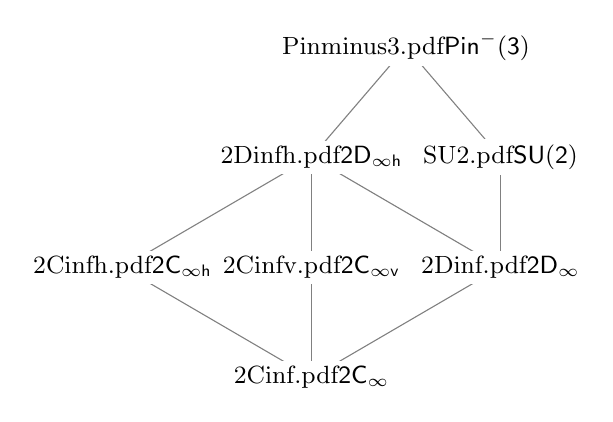
\begin{tikzpicture}[x=1cm, y=1cm, every node/.style={fill=white, font=\small, inner sep=2pt}]
\draw[black!50, line width=0.4pt] (0,0) -- (-2.4,1.4);
\draw[black!50, line width=0.4pt] (0,0) -- (0,1.4);
\draw[black!50, line width=0.4pt] (0,0) -- (2.4,1.4);
\draw[black!50, line width=0.4pt] (-2.4,1.4) -- (0,2.8);
\draw[black!50, line width=0.4pt] (0,1.4) -- (0,2.8);
\draw[black!50, line width=0.4pt] (2.4,1.4) -- (0,2.8);
\draw[black!50, line width=0.4pt] (2.4,1.4) -- (2.4,2.8);
\draw[black!50, line width=0.4pt] (0,2.8) -- (1.2,4.2);
\draw[black!50, line width=0.4pt] (2.4,2.8) -- (1.2,4.2);
\node at (0,0) {\href{2Cinf.pdf}{\textcolor{black}{$\grp{2C_{\infty }}$}}};
\node at (-2.4,1.4) {\href{2Cinfh.pdf}{\textcolor{black}{$\grp{2C_{\infty h}}$}}};
\node at (0,1.4) {\href{2Cinfv.pdf}{\textcolor{black}{$\grp{2C_{\infty v}}$}}};
\node at (2.4,1.4) {\href{2Dinf.pdf}{\textcolor{black}{$\grp{2D_{\infty }}$}}};
\node at (0,2.8) {\href{2Dinfh.pdf}{\textcolor{black}{$\grp{2D_{\infty h}}$}}};
\node at (2.4,2.8) {\href{SU2.pdf}{\textcolor{black}{$\grp{SU(2)}$}}};
\node at (1.2,4.2) {\href{Pinminus3.pdf}{\textcolor{black}{$\grp{Pin^{-}(3)}$}}};
\end{tikzpicture}\end{center}
\leavevmode\label{n:group.H}The table lists the closed subgroups $\grp{H}$ other than $\grp{Pin^{-}(3)}$ up to conjugacy in $\grp{Pin^{-}(3)}$, one in each row: the continuous subgroups, then the preimages and the sections of each family, then the exceptional preimages. A row with $N$ in its symbol stands for every $N$ of its range, and its entries are functions of $N$. \label{n:head.subgroup}\label{n:head.order}\label{n:head.conjugates}\label{n:head.normal}A row gives the representative $\grp{H}$ of a class of subgroups (subgrp), its order, the number of subgroups in the class (conjugates) and whether $\grp{H}$ is normal. \label{n:group.normalizer}\label{n:group.centralizer}It also gives the normalizer $\grp{N}_{\hairsp \grp{Pin^{-}(3)}}(\grp{H})$ and the centralizer $\grp{C}_{\hairsp \grp{Pin^{-}(3)}}(\grp{H})$ in $\grp{Pin^{-}(3)}$ (\texttt{normalizer}, \texttt{centralizer}). This catalogue holds the members with $N \le 12$ (\texttt{data/double\symbol{95}groups.json}), whose records give these normalizers and centralizers (\texttt{subgroup\symbol{95}classes}). A subgroup's other names in its \href{Pinminus3.pdf}{$\grp{Pin^{-}(3)}$}-conjugacy class follow $\samecls$ (\href{../../CONVENTIONS.pdf}{CONVENTIONS.pdf}, section \href{../../CONVENTIONS.pdf\#conv.20.2}{20.2}).
{\small\begin{longtable}{@{}lrrlll@{}}\toprule
subgrp & order & conjugates & normal & $\grp{N}_{\hairsp \grp{Pin^{-}(3)}}(\grp{H})$ & $\grp{C}_{\hairsp \grp{Pin^{-}(3)}}(\grp{H})$\\\midrule\endhead
\bottomrule\endfoot\endlastfoot
\href{2Cinf.pdf}{$\grp{2C_{\infty }}$} & $\infty$ & $\infty$ & no & \href{2Dinfh.pdf}{$\grp{2D_{\infty h}}$} & \href{2Cinfh.pdf}{$\grp{2C_{\infty h}}$}\\*
\href{2Cinfh.pdf}{$\grp{2C_{\infty h}}$} & $\infty$ & $\infty$ & no & \href{2Dinfh.pdf}{$\grp{2D_{\infty h}}$} & \href{2Cinfh.pdf}{$\grp{2C_{\infty h}}$}\\
\href{2Cinfv.pdf}{$\grp{2C_{\infty v}}$} & $\infty$ & $\infty$ & no & \href{2Dinfh.pdf}{$\grp{2D_{\infty h}}$} & \href{2S2.pdf}{$\grp{2C_{i}}$}\\
\href{2Dinf.pdf}{$\grp{2D_{\infty }}$} & $\infty$ & $\infty$ & no & \href{2Dinfh.pdf}{$\grp{2D_{\infty h}}$} & \href{2S2.pdf}{$\grp{2C_{i}}$}\\
\href{2Dinfh.pdf}{$\grp{2D_{\infty h}}$} & $\infty$ & $\infty$ & no & \href{2Dinfh.pdf}{$\grp{2D_{\infty h}}$} & \href{2S2.pdf}{$\grp{2C_{i}}$}\\
\href{SU2.pdf}{$\grp{SU(2)}$} & $\infty$ & 1 & yes & \href{Pinminus3.pdf}{$\grp{Pin^{-}(3)}$} & \href{2S2.pdf}{$\grp{2C_{i}}$}\\
\grouprule{0pt}{\lightrulewidth}
\href{2C1.pdf}{$\grp{2C_{1}}$} & 2 & 1 & yes & \href{Pinminus3.pdf}{$\grp{Pin^{-}(3)}$} & \href{Pinminus3.pdf}{$\grp{Pin^{-}(3)}$}\\
\href{2C2.pdf}{$\grp{2C_{2}}$} $\samecls$ \href{2D1.pdf}{$\grp{2D_{1}}$} & 4 & $\infty$ & no & \href{2Dinfh.pdf}{$\grp{2D_{\infty h}}$} & \href{2Cinfh.pdf}{$\grp{2C_{\infty h}}$}\\
$\grp{2C_{\mathnormal{N}}}$, $N \ge 3$ & $2N$ & $\infty$ & no & \href{2Dinfh.pdf}{$\grp{2D_{\infty h}}$} & \href{2Cinfh.pdf}{$\grp{2C_{\infty h}}$}\\
\href{C1.pdf}{$\grp{C_{1}}$} & 1 & 1 & yes & \href{Pinminus3.pdf}{$\grp{Pin^{-}(3)}$} & \href{Pinminus3.pdf}{$\grp{Pin^{-}(3)}$}\\
$\grp{C_{\mathnormal{N}}}$, $N \ge 3$ odd & $N$ & $\infty$ & no & \href{2Dinfh.pdf}{$\grp{2D_{\infty h}}$} & \href{2Cinfh.pdf}{$\grp{2C_{\infty h}}$}\\
\grouprule{0pt}{\lightrulewidth}
\href{2S2.pdf}{$\grp{2C_{i}}$} & 4 & 1 & yes & \href{Pinminus3.pdf}{$\grp{Pin^{-}(3)}$} & \href{Pinminus3.pdf}{$\grp{Pin^{-}(3)}$}\\
$\grp{2S_{2\mathnormal{N}}}$, $N \ge 2$ & $4N$ & $\infty$ & no & \href{2Dinfh.pdf}{$\grp{2D_{\infty h}}$} & \href{2Cinfh.pdf}{$\grp{2C_{\infty h}}$}\\
\href{S2.pdf}{$\grp{C_{i}}$} & 2 & 1 & yes & \href{Pinminus3.pdf}{$\grp{Pin^{-}(3)}$} & \href{Pinminus3.pdf}{$\grp{Pin^{-}(3)}$}\\
$\grp{S_{2\mathnormal{N}}}$, $N \ge 3$ odd & $2N$ & $\infty$ & no & \href{2Dinfh.pdf}{$\grp{2D_{\infty h}}$} & \href{2Cinfh.pdf}{$\grp{2C_{\infty h}}$}\\
\href{S2b.pdf}{$\grp{C_{i}}\secondclass$} & 2 & 1 & yes & \href{Pinminus3.pdf}{$\grp{Pin^{-}(3)}$} & \href{Pinminus3.pdf}{$\grp{Pin^{-}(3)}$}\\
$\grp{S_{2\mathnormal{N}}}\secondclass$, $N \ge 3$ odd & $2N$ & $\infty$ & no & \href{2Dinfh.pdf}{$\grp{2D_{\infty h}}$} & \href{2Cinfh.pdf}{$\grp{2C_{\infty h}}$}\\
\grouprule{0pt}{\lightrulewidth}
\href{2C2h.pdf}{$\grp{2C_{2h}}$} $\samecls$ \href{2D1d.pdf}{$\grp{2D_{1d}}$} & 8 & $\infty$ & no & \href{2Dinfh.pdf}{$\grp{2D_{\infty h}}$} & \href{2Cinfh.pdf}{$\grp{2C_{\infty h}}$}\\
$\grp{2C_{\mathnormal{N}h}}$, $N \ge 3$ & $4N$ & $\infty$ & no & \href{2Dinfh.pdf}{$\grp{2D_{\infty h}}$} & \href{2Cinfh.pdf}{$\grp{2C_{\infty h}}$}\\
\grouprule{0pt}{\lightrulewidth}
\href{2C1v.pdf}{$\grp{2C_{s}}$} $\samecls$ \href{2C1h.pdf}{$\grp{2C_{1h}}$} & 4 & $\infty$ & no & \href{2Dinfh.pdf}{$\grp{2D_{\infty h}}$} & \href{2Cinfh.pdf}{$\grp{2C_{\infty h}}$}\\
\href{2C2v.pdf}{$\grp{2C_{2v}}$} $\samecls$ \href{2D1h.pdf}{$\grp{2D_{1h}}$} & 8 & $\infty$ & no & \href{2D4h.pdf}{$\grp{2D_{4h}}$} & \href{2S2.pdf}{$\grp{2C_{i}}$}\\
$\grp{2C_{\mathnormal{N}v}}$, $N \ge 3$ & $4N$ & $\infty$ & no & $\grp{2D_{2\mathnormal{N}h}}$ & \href{2S2.pdf}{$\grp{2C_{i}}$}\\
\grouprule{0pt}{\lightrulewidth}
\href{2D2.pdf}{$\grp{2D_{2}}$} & 8 & $\infty$ & no & \href{2Oh.pdf}{$\grp{2O_{h}}$} & \href{2S2.pdf}{$\grp{2C_{i}}$}\\
$\grp{2D_{\mathnormal{N}}}$, $N \ge 3$ & $4N$ & $\infty$ & no & $\grp{2D_{2\mathnormal{N}h}}$ & \href{2S2.pdf}{$\grp{2C_{i}}$}\\
\grouprule{0pt}{\lightrulewidth}
\href{2D2h.pdf}{$\grp{2D_{2h}}$} & 16 & $\infty$ & no & \href{2Oh.pdf}{$\grp{2O_{h}}$} & \href{2S2.pdf}{$\grp{2C_{i}}$}\\
$\grp{2D_{\mathnormal{N}h}}$, $N \ge 3$ & $8N$ & $\infty$ & no & $\grp{2D_{2\mathnormal{N}h}}$ & \href{2S2.pdf}{$\grp{2C_{i}}$}\\
\grouprule{0pt}{\lightrulewidth}
$\grp{2D_{\mathnormal{N}d}}$, $N \ge 2$ & $8N$ & $\infty$ & no & $\grp{2D_{2\mathnormal{N}h}}$ & \href{2S2.pdf}{$\grp{2C_{i}}$}\\
\grouprule{0pt}{\lightrulewidth}
\href{2T.pdf}{$\grp{2T}$} & 24 & $\infty$ & no & \href{2Oh.pdf}{$\grp{2O_{h}}$} & \href{2S2.pdf}{$\grp{2C_{i}}$}\\
\href{2Th.pdf}{$\grp{2T_{h}}$} & 48 & $\infty$ & no & \href{2Oh.pdf}{$\grp{2O_{h}}$} & \href{2S2.pdf}{$\grp{2C_{i}}$}\\
\href{2Td.pdf}{$\grp{2T_{d}}$} & 48 & $\infty$ & no & \href{2Oh.pdf}{$\grp{2O_{h}}$} & \href{2S2.pdf}{$\grp{2C_{i}}$}\\
\href{2O.pdf}{$\grp{2O}$} & 48 & $\infty$ & no & \href{2Oh.pdf}{$\grp{2O_{h}}$} & \href{2S2.pdf}{$\grp{2C_{i}}$}\\
\href{2Oh.pdf}{$\grp{2O_{h}}$} & 96 & $\infty$ & no & \href{2Oh.pdf}{$\grp{2O_{h}}$} & \href{2S2.pdf}{$\grp{2C_{i}}$}\\
\href{2I.pdf}{$\grp{2I}$} & 120 & $\infty$ & no & \href{2Ih.pdf}{$\grp{2I_{h}}$} & \href{2S2.pdf}{$\grp{2C_{i}}$}\\*
\href{2Ih.pdf}{$\grp{2I_{h}}$} & 240 & $\infty$ & no & \href{2Ih.pdf}{$\grp{2I_{h}}$} & \href{2S2.pdf}{$\grp{2C_{i}}$}\\
\bottomrule\end{longtable}}
\needspace{103pt}
\section{Descent of symmetry}\label{s:subduction}
Conventions: \href{../../CONVENTIONS.pdf}{CONVENTIONS.pdf}, sections \href{../../../rotation/CONVENTIONS.pdf\#conv.16.1}{16.1} and \href{../../CONVENTIONS.pdf\#conv.29.6}{29.6}.
\leavevmode\label{n:irrep.Gamma.subgroup}Below is the restriction of $\irrJp{J}{p}$ to each closed subgroup $\grp{H}$ of $\grp{Pin^{-}(3)}$ (section~\ref{s:subgroups}) for every half-integer $J$ and both parities (\texttt{subduction\symbol{95}rules}). At integer $J$ the restriction is that of \href{../../../rotation/data/pdf/O3.pdf}{$\grp{O(3)}$}, in its section Descent of symmetry. For an axial $\grp{H}$ the restriction at half-integer $J$ is the direct sum, over the kets $\jm{J}{m}$, of the terms of the first true case of its rule. For \href{2Cinfv.pdf}{$\grp{2C_{\infty v}}$}, \href{2Dinf.pdf}{$\grp{2D_{\infty }}$}, \href{2Dinfh.pdf}{$\grp{2D_{\infty h}}$} and the preimages of $\grp{C_{\mathnormal{N}v}}$, $\grp{D_{\mathnormal{N}}}$, $\grp{D_{\mathnormal{N}h}}$ and $\grp{D_{\mathnormal{N}d}}$, the sum runs over the pairs $\jm{J}{\pm m}$. \label{n:index.residue}In the rules, $q = m \bmod N$. However, in the preimages of $\grp{S_{2\mathnormal{N}}}$ and $\grp{D_{\mathnormal{N}d}}$ with $N$ even and of $\grp{C_{\mathnormal{N}h}}$ and $\grp{D_{\mathnormal{N}h}}$ with $N$ odd, $q$ is taken modulo $2N$, shifted by $N$ at $p = -1$. The map $(U, \varepsilon) \mapsto U$ carries these preimages onto $\grp{2C_{2\mathnormal{N}}}$ or $\grp{2D_{2\mathnormal{N}}}$. An irrep is named by the least $J$ at which it occurs in the restriction of $\irrJp{J}{p}$, where $p = -1$ for the tag $\ptag{u}$ and $p = +1$ otherwise (\href{../../CONVENTIONS.pdf}{CONVENTIONS.pdf}, section \href{../../CONVENTIONS.pdf\#conv.23.2}{23.2}). In the rules of a family, the terms are irreps of the member, labeled as in \href{../../CONVENTIONS.pdf}{CONVENTIONS.pdf}, sections \href{../../../rotation/CONVENTIONS.pdf\#conv.6.1}{6.1} and \href{../../CONVENTIONS.pdf\#conv.23.2}{23.2}. The terms of a rule whose subgroup contains $\elt{\lift{i}}$, which acts on $\irrJp{J}{p}$ as $p$, are written at $p = +1$. A section over $\grp{C_{\mathnormal{N}}}$ or $\grp{S_{2\mathnormal{N}}}$ ($N$ odd) is restricted as its preimage, with each spinor irrep renamed by the section's record (\href{../../CONVENTIONS.pdf}{CONVENTIONS.pdf}, section \href{../../CONVENTIONS.pdf\#conv.27}{27}). \label{n:function.multiplicity}\label{n:index.generating.variable}\label{n:function.generating}\label{n:function.generating.numerator}\label{n:irrep.Delta}The multiplicity $b_\Lambda(J)$ of an irrep $\Lambda$ of $\grp{H}$ at $p = +1$ is the coefficient of $t^{2J}$ in its generating function $H_\Lambda(t) = \sum_{J\ge1/2} b_\Lambda(J)\,t^{2J}$. The documents of the subgroups use this definition in their section Multiplicities and allowed $m$. At $p = -1$ the multiplicity of $\Lambda$ is that of the product of $\Lambda$ and the determinant character of $\grp{H}$. In the generating functions, $k$ is the subscript of an irrep $\irr{e}_{k}$, and $n$ the index of a family of irreps of a continuous subgroup. The document of each preimage except the members with $N > 12$ lists the restrictions $J$ by $J$ at both parities, in its section Subduction from \href{Pinminus3.pdf}{$\grp{Pin^{-}(3)}$}.
\needspace{95pt}
\paragraph{Continuous subgroups.}
{\small\renewcommand{\arraystretch}{1.6}\setlength{\fillwidth}{\textwidth}\addtolength{\fillwidth}{-2\tabcolsep}\setlength{\colwidth}{0pt}\cellmax{$\irrJp{J}{p}$}\cellmax{$H_\Lambda(t)$}\addtolength{\fillwidth}{-\colwidth}\setlength{\colwidth}{0pt}\cellmax{$\bigoplus_{m=-J}^{J}\Lambda_m$, $\Lambda_m$ on $\jm{J}{m}$: $\conjpair{1}\irr{e}_{m,\ptag{g}}$ if $m > 0$, $\conjpair{2}\irr{e}_{-m,\ptag{g}}$ if $m < 0$; at $p = -1$ the same with $\ptag{u}$ for $\ptag{g}$}\cellmax{$\bigoplus_{m=1/2}^{J}\Lambda_m$, $\Lambda_m$ on the pair $\jm{J}{\pm m}$: $\irr{e}_{m,\ptag{g}}$ if $m > 0$; at $p = -1$ the same with $\ptag{u}$ for $\ptag{g}$}\cellmax{$\bigoplus_{m=-J}^{J}\Lambda_m$, $\Lambda_m$ on $\jm{J}{m}$: $\conjpair{1}\irr{e}_{m}$ if $m > 0$, $\conjpair{2}\irr{e}_{-m}$ if $m < 0$; independent of $p$}\cellmax{$\bigoplus_{m=1/2}^{J}\Lambda_m$, $\Lambda_m$ on the pair $\jm{J}{\pm m}$: $\irr{e}_{m}$ if $m > 0$; independent of $p$}\cellmax{$t^{2n}/(1-t^{2})$ for $\conjpair{1}\irr{e}_{n,\ptag{g}}$ and $\conjpair{2}\irr{e}_{n,\ptag{g}}$, $0$ for $\conjpair{1}\irr{e}_{n,\ptag{u}}$ and $\conjpair{2}\irr{e}_{n,\ptag{u}}$}\cellmax{$t^{2n}/(1-t^{2})$ for $\irr{e}_{n,\ptag{g}}$, $0$ for $\irr{e}_{n,\ptag{u}}$}\cellmax{$t^{2n}/(1-t^{2})$ for $\conjpair{1}\irr{e}_{n}$ and $\conjpair{2}\irr{e}_{n}$}\cellmax{$\irrJ{J}$, independent of $p$}\cellmax{$t^{2n}/(1-t^{2})$ for $\irr{e}_{n}$}\fillcap\begin{longtable}{@{}l>{\raggedright\arraybackslash}p{\fillwidth}@{}}\toprule
\multicolumn{2}{@{}c@{}}{\href{2Cinf.pdf}{$\grp{2C_{\infty }}$}}\\*
$\irrJp{J}{p}$ & $\bigoplus_{m=-J}^{J}\Lambda_m$, $\Lambda_m$ on $\jm{J}{m}$: $\conjpair{1}\irr{e}_{m}$ if $m > 0$, $\conjpair{2}\irr{e}_{-m}$ if $m < 0$; independent of $p$\\*
$H_\Lambda(t)$ & $t^{2n}/(1-t^{2})$ for $\conjpair{1}\irr{e}_{n}$ and $\conjpair{2}\irr{e}_{n}$\\
\grouprule{0pt}{\lightrulewidth}
\multicolumn{2}{@{}c@{}}{\href{2Cinfh.pdf}{$\grp{2C_{\infty h}}$}}\\*
$\irrJp{J}{p}$ & $\bigoplus_{m=-J}^{J}\Lambda_m$, $\Lambda_m$ on $\jm{J}{m}$: $\conjpair{1}\irr{e}_{m,\ptag{g}}$ if $m > 0$, $\conjpair{2}\irr{e}_{-m,\ptag{g}}$ if $m < 0$; at $p = -1$ the same with $\ptag{u}$ for $\ptag{g}$\\*
$H_\Lambda(t)$ & $t^{2n}/(1-t^{2})$ for $\conjpair{1}\irr{e}_{n,\ptag{g}}$ and $\conjpair{2}\irr{e}_{n,\ptag{g}}$, $0$ for $\conjpair{1}\irr{e}_{n,\ptag{u}}$ and $\conjpair{2}\irr{e}_{n,\ptag{u}}$\\
\grouprule{0pt}{\lightrulewidth}
\multicolumn{2}{@{}c@{}}{\href{2Cinfv.pdf}{$\grp{2C_{\infty v}}$}}\\*
$\irrJp{J}{p}$ & $\bigoplus_{m=1/2}^{J}\Lambda_m$, $\Lambda_m$ on the pair $\jm{J}{\pm m}$: $\irr{e}_{m}$ if $m > 0$; independent of $p$\\*
$H_\Lambda(t)$ & $t^{2n}/(1-t^{2})$ for $\irr{e}_{n}$\\
\grouprule{0pt}{\lightrulewidth}
\multicolumn{2}{@{}c@{}}{\href{2Dinf.pdf}{$\grp{2D_{\infty }}$}}\\*
$\irrJp{J}{p}$ & $\bigoplus_{m=1/2}^{J}\Lambda_m$, $\Lambda_m$ on the pair $\jm{J}{\pm m}$: $\irr{e}_{m}$ if $m > 0$; independent of $p$\\*
$H_\Lambda(t)$ & $t^{2n}/(1-t^{2})$ for $\irr{e}_{n}$\\
\grouprule{0pt}{\lightrulewidth}
\multicolumn{2}{@{}c@{}}{\href{2Dinfh.pdf}{$\grp{2D_{\infty h}}$}}\\*
$\irrJp{J}{p}$ & $\bigoplus_{m=1/2}^{J}\Lambda_m$, $\Lambda_m$ on the pair $\jm{J}{\pm m}$: $\irr{e}_{m,\ptag{g}}$ if $m > 0$; at $p = -1$ the same with $\ptag{u}$ for $\ptag{g}$\\*
$H_\Lambda(t)$ & $t^{2n}/(1-t^{2})$ for $\irr{e}_{n,\ptag{g}}$, $0$ for $\irr{e}_{n,\ptag{u}}$\\
\grouprule{0pt}{\lightrulewidth}
\multicolumn{2}{@{}c@{}}{\href{SU2.pdf}{$\grp{SU(2)}$}}\\*
$\irrJp{J}{p}$ & $\irrJ{J}$, independent of $p$\\
\bottomrule\end{longtable}}

\needspace{95pt}
\paragraph{Subduction to the $\grp{2C_{\mathnormal{N}}}$ family.}
{\small\renewcommand{\arraystretch}{1.6}\setlength{\fillwidth}{\textwidth}\addtolength{\fillwidth}{-2\tabcolsep}\setlength{\colwidth}{0pt}\cellmax{$\irrJp{J}{p}$}\cellmax{$H_\Lambda(t)$}\addtolength{\fillwidth}{-\colwidth}\setlength{\colwidth}{0pt}\cellmax{$\bigoplus_{m=-J}^{J}\Lambda_m$, $\Lambda_m$ on $\jm{J}{m}$: $\conjpair{1}\irr{e}_{q}$ if $0 < q < N/2$, $\irr{a}_{N/2}$ if $q = N/2$, $\conjpair{2}\irr{e}_{N-q}$ if $N/2 < q < N$; $q = m \bmod N$; independent of $p$}\cellmax{$P_\Lambda(t)/((1-t^{2})(1-t^{2N}))$, $P_\Lambda(t)$: $t^{2k} + t^{2N-2k}$ for $\conjpair{1}\irr{e}_{k}$ and $\conjpair{2}\irr{e}_{k}$ ($0 < k < N/2$), $2t^{N}$ for $\irr{a}_{N/2}$ ($N$ odd)}\fillcap\begin{longtable}{@{}l>{\raggedright\arraybackslash}p{\fillwidth}@{}}\toprule
\multicolumn{2}{@{}c@{}}{every $N$}\\*
$\irrJp{J}{p}$ & $\bigoplus_{m=-J}^{J}\Lambda_m$, $\Lambda_m$ on $\jm{J}{m}$: $\conjpair{1}\irr{e}_{q}$ if $0 < q < N/2$, $\irr{a}_{N/2}$ if $q = N/2$, $\conjpair{2}\irr{e}_{N-q}$ if $N/2 < q < N$; $q = m \bmod N$; independent of $p$\\*
$H_\Lambda(t)$ & $P_\Lambda(t)/((1-t^{2})(1-t^{2N}))$, $P_\Lambda(t)$: $t^{2k} + t^{2N-2k}$ for $\conjpair{1}\irr{e}_{k}$ and $\conjpair{2}\irr{e}_{k}$ ($0 < k < N/2$), $2t^{N}$ for $\irr{a}_{N/2}$ ($N$ odd)\\
\bottomrule\end{longtable}}

\needspace{95pt}
\paragraph{Subduction to the $\grp{2S_{2\mathnormal{N}}}$ family.}
{\small\renewcommand{\arraystretch}{1.6}\setlength{\fillwidth}{\textwidth}\addtolength{\fillwidth}{-2\tabcolsep}\setlength{\colwidth}{0pt}\cellmax{$\irrJp{J}{p}$}\cellmax{$H_\Lambda(t)$}\addtolength{\fillwidth}{-\colwidth}\setlength{\colwidth}{0pt}\cellmax{$P_\Lambda(t)/((1-t^{2})(1-t^{2N}))$, $P_\Lambda(t)$: $t^{2k} + t^{2N-2k}$ for $\conjpair{1}\irr{e}_{k,\ptag{g}}$ and $\conjpair{2}\irr{e}_{k,\ptag{g}}$ ($0 < k < N/2$), $2t^{N}$ for $\irr{a}_{N/2,\ptag{g}}$ ($N$ odd), $0$ for $\conjpair{1}\irr{e}_{k,\ptag{u}}$ and $\conjpair{2}\irr{e}_{k,\ptag{u}}$ ($0 < k < N/2$), $0$ for $\irr{a}_{N/2,\ptag{u}}$ ($N$ odd)}\cellmax{$\bigoplus_{m=-J}^{J}\Lambda_m$, $\Lambda_m$ on $\jm{J}{m}$: $\conjpair{1}\irr{e}_{q,\ptag{g}}$ if $0 < q < N/2$, $\irr{a}_{N/2,\ptag{g}}$ if $q = N/2$, $\conjpair{2}\irr{e}_{N-q,\ptag{g}}$ if $N/2 < q < N$; at $p = -1$ the same with $\ptag{u}$ for $\ptag{g}$; $q = m \bmod N$}\cellmax{$\bigoplus_{m=-J}^{J}\Lambda_m$, $\Lambda_m$ on $\jm{J}{m}$: $\conjpair{1}\irr{e}_{\min(q,2N-q)}$ if $q \bmod N < N/2$, $\conjpair{2}\irr{e}_{\min(q,2N-q)}$ if $q \bmod N > N/2$; $q = m \bmod 2N$ at $p = +1$ and $m + N \bmod 2N$ at $p = -1$}\cellmax{$P_\Lambda(t)/((1-t^{2})(1-t^{4N}))$, $P_\Lambda(t)$: $t^{2k} + t^{4N-2k}$ for $\conjpair{1}\irr{e}_{k}$ and $\conjpair{2}\irr{e}_{k}$ ($0 < k < N$)}\fillcap\begin{longtable}{@{}l>{\raggedright\arraybackslash}p{\fillwidth}@{}}\toprule
\multicolumn{2}{@{}c@{}}{odd $N$}\\*
$\irrJp{J}{p}$ & $\bigoplus_{m=-J}^{J}\Lambda_m$, $\Lambda_m$ on $\jm{J}{m}$: $\conjpair{1}\irr{e}_{q,\ptag{g}}$ if $0 < q < N/2$, $\irr{a}_{N/2,\ptag{g}}$ if $q = N/2$, $\conjpair{2}\irr{e}_{N-q,\ptag{g}}$ if $N/2 < q < N$; at $p = -1$ the same with $\ptag{u}$ for $\ptag{g}$; $q = m \bmod N$\\*
$H_\Lambda(t)$ & $P_\Lambda(t)/((1-t^{2})(1-t^{2N}))$, $P_\Lambda(t)$: $t^{2k} + t^{2N-2k}$ for $\conjpair{1}\irr{e}_{k,\ptag{g}}$ and $\conjpair{2}\irr{e}_{k,\ptag{g}}$ ($0 < k < N/2$), $2t^{N}$ for $\irr{a}_{N/2,\ptag{g}}$ ($N$ odd), $0$ for $\conjpair{1}\irr{e}_{k,\ptag{u}}$ and $\conjpair{2}\irr{e}_{k,\ptag{u}}$ ($0 < k < N/2$), $0$ for $\irr{a}_{N/2,\ptag{u}}$ ($N$ odd)\\
\grouprule{0pt}{\lightrulewidth}
\multicolumn{2}{@{}c@{}}{even $N$}\\*
$\irrJp{J}{p}$ & $\bigoplus_{m=-J}^{J}\Lambda_m$, $\Lambda_m$ on $\jm{J}{m}$: $\conjpair{1}\irr{e}_{\min(q,2N-q)}$ if $q \bmod N < N/2$, $\conjpair{2}\irr{e}_{\min(q,2N-q)}$ if $q \bmod N > N/2$; $q = m \bmod 2N$ at $p = +1$ and $m + N \bmod 2N$ at $p = -1$\\*
$H_\Lambda(t)$ & $P_\Lambda(t)/((1-t^{2})(1-t^{4N}))$, $P_\Lambda(t)$: $t^{2k} + t^{4N-2k}$ for $\conjpair{1}\irr{e}_{k}$ and $\conjpair{2}\irr{e}_{k}$ ($0 < k < N$)\\
\bottomrule\end{longtable}}

\needspace{95pt}
\paragraph{Subduction to the $\grp{2C_{\mathnormal{N}h}}$ family.}
{\small\renewcommand{\arraystretch}{1.6}\setlength{\fillwidth}{\textwidth}\addtolength{\fillwidth}{-2\tabcolsep}\setlength{\colwidth}{0pt}\cellmax{$\irrJp{J}{p}$}\cellmax{$H_\Lambda(t)$}\addtolength{\fillwidth}{-\colwidth}\setlength{\colwidth}{0pt}\cellmax{$\bigoplus_{m=-J}^{J}\Lambda_m$, $\Lambda_m$ on $\jm{J}{m}$: $\irr{e}_{\min(q,2N-q)}'$; with $''$ for $'$ on the kets where $p(-1)^{m-1/2} = -1$; $q = m \bmod 2N$ at $p = +1$ and $m + N \bmod 2N$ at $p = -1$}\cellmax{$P_\Lambda(t)/((1-t^{2})(1-t^{2N}))$, $P_\Lambda(t)$: $t^{2k} + t^{2N-2k}$ for $\conjpair{1}\irr{e}_{k,\ptag{g}}$ and $\conjpair{2}\irr{e}_{k,\ptag{g}}$ ($0 < k < N/2$), $0$ for $\conjpair{1}\irr{e}_{k,\ptag{u}}$ and $\conjpair{2}\irr{e}_{k,\ptag{u}}$ ($0 < k < N/2$)}\cellmax{$\bigoplus_{m=-J}^{J}\Lambda_m$, $\Lambda_m$ on $\jm{J}{m}$: $\conjpair{1}\irr{e}_{q,\ptag{g}}$ if $0 < q < N/2$, $\conjpair{2}\irr{e}_{N-q,\ptag{g}}$ if $N/2 < q < N$; at $p = -1$ the same with $\ptag{u}$ for $\ptag{g}$; $q = m \bmod N$}\cellmax{$P_\Lambda(t)/((1-t^{2})(1-t^{4N}))$, $P_\Lambda(t)$: $t^{2k} + t^{4N-2k}$ for $\irr{e}_{k}'$ and $\irr{e}_{k}''$ ($0 < k < N$)}\fillcap\begin{longtable}{@{}l>{\raggedright\arraybackslash}p{\fillwidth}@{}}\toprule
\multicolumn{2}{@{}c@{}}{odd $N$}\\*
$\irrJp{J}{p}$ & $\bigoplus_{m=-J}^{J}\Lambda_m$, $\Lambda_m$ on $\jm{J}{m}$: $\irr{e}_{\min(q,2N-q)}'$; with $''$ for $'$ on the kets where $p(-1)^{m-1/2} = -1$; $q = m \bmod 2N$ at $p = +1$ and $m + N \bmod 2N$ at $p = -1$\\*
$H_\Lambda(t)$ & $P_\Lambda(t)/((1-t^{2})(1-t^{4N}))$, $P_\Lambda(t)$: $t^{2k} + t^{4N-2k}$ for $\irr{e}_{k}'$ and $\irr{e}_{k}''$ ($0 < k < N$)\\
\grouprule{0pt}{\lightrulewidth}
\multicolumn{2}{@{}c@{}}{even $N$}\\*
$\irrJp{J}{p}$ & $\bigoplus_{m=-J}^{J}\Lambda_m$, $\Lambda_m$ on $\jm{J}{m}$: $\conjpair{1}\irr{e}_{q,\ptag{g}}$ if $0 < q < N/2$, $\conjpair{2}\irr{e}_{N-q,\ptag{g}}$ if $N/2 < q < N$; at $p = -1$ the same with $\ptag{u}$ for $\ptag{g}$; $q = m \bmod N$\\*
$H_\Lambda(t)$ & $P_\Lambda(t)/((1-t^{2})(1-t^{2N}))$, $P_\Lambda(t)$: $t^{2k} + t^{2N-2k}$ for $\conjpair{1}\irr{e}_{k,\ptag{g}}$ and $\conjpair{2}\irr{e}_{k,\ptag{g}}$ ($0 < k < N/2$), $0$ for $\conjpair{1}\irr{e}_{k,\ptag{u}}$ and $\conjpair{2}\irr{e}_{k,\ptag{u}}$ ($0 < k < N/2$)\\
\bottomrule\end{longtable}}

\needspace{95pt}
\paragraph{Subduction to the $\grp{2C_{\mathnormal{N}v}}$ family.}
{\small\renewcommand{\arraystretch}{1.6}\setlength{\fillwidth}{\textwidth}\addtolength{\fillwidth}{-2\tabcolsep}\setlength{\colwidth}{0pt}\cellmax{$\irrJp{J}{p}$}\cellmax{$H_\Lambda(t)$}\addtolength{\fillwidth}{-\colwidth}\setlength{\colwidth}{0pt}\cellmax{$\bigoplus_{m=1/2}^{J}\Lambda_m$, $\Lambda_m$ on the pair $\jm{J}{\pm m}$: $\irr{e}_{\min(q,N-q)}$ if $q \ne N/2$, $\conjpair{1}\irr{e}_{N/2}\oplus \conjpair{2}\irr{e}_{N/2}$ if $q = N/2$; $q = m \bmod N$; independent of $p$}\cellmax{$P_\Lambda(t)/((1-t^{2})(1-t^{2N}))$, $P_\Lambda(t)$: $t^{2k} + t^{2N-2k}$ for $\irr{e}_{k}$ ($0 < k < N/2$), $t^{N}$ for $\conjpair{1}\irr{e}_{N/2}$ and $\conjpair{2}\irr{e}_{N/2}$ ($N$ odd)}\fillcap\begin{longtable}{@{}l>{\raggedright\arraybackslash}p{\fillwidth}@{}}\toprule
\multicolumn{2}{@{}c@{}}{every $N$}\\*
$\irrJp{J}{p}$ & $\bigoplus_{m=1/2}^{J}\Lambda_m$, $\Lambda_m$ on the pair $\jm{J}{\pm m}$: $\irr{e}_{\min(q,N-q)}$ if $q \ne N/2$, $\conjpair{1}\irr{e}_{N/2}\oplus \conjpair{2}\irr{e}_{N/2}$ if $q = N/2$; $q = m \bmod N$; independent of $p$\\*
$H_\Lambda(t)$ & $P_\Lambda(t)/((1-t^{2})(1-t^{2N}))$, $P_\Lambda(t)$: $t^{2k} + t^{2N-2k}$ for $\irr{e}_{k}$ ($0 < k < N/2$), $t^{N}$ for $\conjpair{1}\irr{e}_{N/2}$ and $\conjpair{2}\irr{e}_{N/2}$ ($N$ odd)\\
\bottomrule\end{longtable}}

\needspace{95pt}
\paragraph{Subduction to the $\grp{2D_{\mathnormal{N}}}$ family.}
{\small\renewcommand{\arraystretch}{1.6}\setlength{\fillwidth}{\textwidth}\addtolength{\fillwidth}{-2\tabcolsep}\setlength{\colwidth}{0pt}\cellmax{$\irrJp{J}{p}$}\cellmax{$H_\Lambda(t)$}\addtolength{\fillwidth}{-\colwidth}\setlength{\colwidth}{0pt}\cellmax{$\bigoplus_{m=1/2}^{J}\Lambda_m$, $\Lambda_m$ on the pair $\jm{J}{\pm m}$: $\irr{e}_{\min(q,N-q)}$ if $q \ne N/2$, $\conjpair{1}\irr{e}_{N/2}\oplus \conjpair{2}\irr{e}_{N/2}$ if $q = N/2$; $q = m \bmod N$; independent of $p$}\cellmax{$P_\Lambda(t)/((1-t^{2})(1-t^{2N}))$, $P_\Lambda(t)$: $t^{2k} + t^{2N-2k}$ for $\irr{e}_{k}$ ($0 < k < N/2$), $t^{N}$ for $\conjpair{1}\irr{e}_{N/2}$ and $\conjpair{2}\irr{e}_{N/2}$ ($N$ odd)}\fillcap\begin{longtable}{@{}l>{\raggedright\arraybackslash}p{\fillwidth}@{}}\toprule
\multicolumn{2}{@{}c@{}}{every $N \ge 2$}\\*
$\irrJp{J}{p}$ & $\bigoplus_{m=1/2}^{J}\Lambda_m$, $\Lambda_m$ on the pair $\jm{J}{\pm m}$: $\irr{e}_{\min(q,N-q)}$ if $q \ne N/2$, $\conjpair{1}\irr{e}_{N/2}\oplus \conjpair{2}\irr{e}_{N/2}$ if $q = N/2$; $q = m \bmod N$; independent of $p$\\*
$H_\Lambda(t)$ & $P_\Lambda(t)/((1-t^{2})(1-t^{2N}))$, $P_\Lambda(t)$: $t^{2k} + t^{2N-2k}$ for $\irr{e}_{k}$ ($0 < k < N/2$), $t^{N}$ for $\conjpair{1}\irr{e}_{N/2}$ and $\conjpair{2}\irr{e}_{N/2}$ ($N$ odd)\\
\bottomrule\end{longtable}}

\needspace{95pt}
\paragraph{Subduction to the $\grp{2D_{\mathnormal{N}h}}$ family.}
{\small\renewcommand{\arraystretch}{1.6}\setlength{\fillwidth}{\textwidth}\addtolength{\fillwidth}{-2\tabcolsep}\setlength{\colwidth}{0pt}\cellmax{$\irrJp{J}{p}$}\cellmax{$H_\Lambda(t)$}\addtolength{\fillwidth}{-\colwidth}\setlength{\colwidth}{0pt}\cellmax{$P_\Lambda(t)/((1-t^{2})(1-t^{2N}))$, $P_\Lambda(t)$: $t^{2k} + t^{2N-2k}$ for $\irr{e}_{k,\ptag{g}}$ ($0 < k < N/2$), $0$ for $\irr{e}_{k,\ptag{u}}$ ($0 < k < N/2$)}\cellmax{$\bigoplus_{m=1/2}^{J}\Lambda_m$, $\Lambda_m$ on the pair $\jm{J}{\pm m}$: $\irr{e}_{\min(q,N-q),\ptag{g}}$; at $p = -1$ the same with $\ptag{u}$ for $\ptag{g}$; $q = m \bmod N$}\cellmax{$\bigoplus_{m=1/2}^{J}\Lambda_m$, $\Lambda_m$ on the pair $\jm{J}{\pm m}$: $\irr{e}_{\min(q,2N-q)}$; $q = m \bmod 2N$ at $p = +1$ and $m + N \bmod 2N$ at $p = -1$}\cellmax{$P_\Lambda(t)/((1-t^{2})(1-t^{4N}))$, $P_\Lambda(t)$: $t^{2k} + t^{4N-2k}$ for $\irr{e}_{k}$ ($0 < k < N$)}\fillcap\begin{longtable}{@{}l>{\raggedright\arraybackslash}p{\fillwidth}@{}}\toprule
\multicolumn{2}{@{}c@{}}{odd $N$}\\*
$\irrJp{J}{p}$ & $\bigoplus_{m=1/2}^{J}\Lambda_m$, $\Lambda_m$ on the pair $\jm{J}{\pm m}$: $\irr{e}_{\min(q,2N-q)}$; $q = m \bmod 2N$ at $p = +1$ and $m + N \bmod 2N$ at $p = -1$\\*
$H_\Lambda(t)$ & $P_\Lambda(t)/((1-t^{2})(1-t^{4N}))$, $P_\Lambda(t)$: $t^{2k} + t^{4N-2k}$ for $\irr{e}_{k}$ ($0 < k < N$)\\
\grouprule{0pt}{\lightrulewidth}
\multicolumn{2}{@{}c@{}}{even $N$}\\*
$\irrJp{J}{p}$ & $\bigoplus_{m=1/2}^{J}\Lambda_m$, $\Lambda_m$ on the pair $\jm{J}{\pm m}$: $\irr{e}_{\min(q,N-q),\ptag{g}}$; at $p = -1$ the same with $\ptag{u}$ for $\ptag{g}$; $q = m \bmod N$\\*
$H_\Lambda(t)$ & $P_\Lambda(t)/((1-t^{2})(1-t^{2N}))$, $P_\Lambda(t)$: $t^{2k} + t^{2N-2k}$ for $\irr{e}_{k,\ptag{g}}$ ($0 < k < N/2$), $0$ for $\irr{e}_{k,\ptag{u}}$ ($0 < k < N/2$)\\
\bottomrule\end{longtable}}

\needspace{95pt}
\paragraph{Subduction to the $\grp{2D_{\mathnormal{N}d}}$ family.}
{\small\renewcommand{\arraystretch}{1.6}\setlength{\fillwidth}{\textwidth}\addtolength{\fillwidth}{-2\tabcolsep}\setlength{\colwidth}{0pt}\cellmax{$\irrJp{J}{p}$}\cellmax{$H_\Lambda(t)$}\addtolength{\fillwidth}{-\colwidth}\setlength{\colwidth}{0pt}\cellmax{$P_\Lambda(t)/((1-t^{2})(1-t^{2N}))$, $P_\Lambda(t)$: $t^{2k} + t^{2N-2k}$ for $\irr{e}_{k,\ptag{g}}$ ($0 < k < N/2$), $t^{N}$ for $\conjpair{1}\irr{e}_{N/2,\ptag{g}}$ and $\conjpair{2}\irr{e}_{N/2,\ptag{g}}$ ($N$ odd), $0$ for $\irr{e}_{k,\ptag{u}}$ ($0 < k < N/2$), $0$ for $\conjpair{1}\irr{e}_{N/2,\ptag{u}}$ and $\conjpair{2}\irr{e}_{N/2,\ptag{u}}$ ($N$ odd)}\cellmax{$\bigoplus_{m=1/2}^{J}\Lambda_m$, $\Lambda_m$ on the pair $\jm{J}{\pm m}$: $\irr{e}_{\min(q,N-q),\ptag{g}}$ if $q \ne N/2$, $\conjpair{1}\irr{e}_{N/2,\ptag{g}}\oplus \conjpair{2}\irr{e}_{N/2,\ptag{g}}$ if $q = N/2$; at $p = -1$ the same with $\ptag{u}$ for $\ptag{g}$; $q = m \bmod N$}\cellmax{$\bigoplus_{m=1/2}^{J}\Lambda_m$, $\Lambda_m$ on the pair $\jm{J}{\pm m}$: $\irr{e}_{\min(q,2N-q)}$; $q = m \bmod 2N$ at $p = +1$ and $m + N \bmod 2N$ at $p = -1$}\cellmax{$P_\Lambda(t)/((1-t^{2})(1-t^{4N}))$, $P_\Lambda(t)$: $t^{2k} + t^{4N-2k}$ for $\irr{e}_{k}$ ($0 < k < N$)}\fillcap\begin{longtable}{@{}l>{\raggedright\arraybackslash}p{\fillwidth}@{}}\toprule
\multicolumn{2}{@{}c@{}}{odd $N$}\\*
$\irrJp{J}{p}$ & $\bigoplus_{m=1/2}^{J}\Lambda_m$, $\Lambda_m$ on the pair $\jm{J}{\pm m}$: $\irr{e}_{\min(q,N-q),\ptag{g}}$ if $q \ne N/2$, $\conjpair{1}\irr{e}_{N/2,\ptag{g}}\oplus \conjpair{2}\irr{e}_{N/2,\ptag{g}}$ if $q = N/2$; at $p = -1$ the same with $\ptag{u}$ for $\ptag{g}$; $q = m \bmod N$\\*
$H_\Lambda(t)$ & $P_\Lambda(t)/((1-t^{2})(1-t^{2N}))$, $P_\Lambda(t)$: $t^{2k} + t^{2N-2k}$ for $\irr{e}_{k,\ptag{g}}$ ($0 < k < N/2$), $t^{N}$ for $\conjpair{1}\irr{e}_{N/2,\ptag{g}}$ and $\conjpair{2}\irr{e}_{N/2,\ptag{g}}$ ($N$ odd), $0$ for $\irr{e}_{k,\ptag{u}}$ ($0 < k < N/2$), $0$ for $\conjpair{1}\irr{e}_{N/2,\ptag{u}}$ and $\conjpair{2}\irr{e}_{N/2,\ptag{u}}$ ($N$ odd)\\
\grouprule{0pt}{\lightrulewidth}
\multicolumn{2}{@{}c@{}}{even $N$}\\*
$\irrJp{J}{p}$ & $\bigoplus_{m=1/2}^{J}\Lambda_m$, $\Lambda_m$ on the pair $\jm{J}{\pm m}$: $\irr{e}_{\min(q,2N-q)}$; $q = m \bmod 2N$ at $p = +1$ and $m + N \bmod 2N$ at $p = -1$\\*
$H_\Lambda(t)$ & $P_\Lambda(t)/((1-t^{2})(1-t^{4N}))$, $P_\Lambda(t)$: $t^{2k} + t^{4N-2k}$ for $\irr{e}_{k}$ ($0 < k < N$)\\
\bottomrule\end{longtable}}

\needspace{224pt}
\paragraph{Subduction to the exceptional preimages.} \label{n:index.gf.ab}The generating functions are $H_\Lambda(t) = P_\Lambda(t)/((1-t^{a_1})(1-t^{a_2}))$. The exponents $(a_1, a_2)$ are $(4, 6)$ for $\grp{2T}$, $(4, 6)$ for $\grp{2T_{h}}$, $(6, 8)$ for $\grp{2T_{d}}$, $(6, 8)$ for $\grp{2O}$, $(6, 8)$ for $\grp{2O_{h}}$, $(10, 12)$ for $\grp{2I}$ and $(10, 12)$ for $\grp{2I_{h}}$.
{\small\begin{longtable}{@{}ll@{\hspace{18pt}}ll@{}}\toprule
$\Lambda$ & $P_\Lambda(t)$ & $\Lambda$ & $P_\Lambda(t)$\\\midrule\endhead
\bottomrule\endfoot\endlastfoot
\multicolumn{2}{@{}c@{\hspace{18pt}}}{\href{2T.pdf}{$\grp{2T}$}} & \multicolumn{2}{@{}c@{}}{\href{2Td.pdf}{$\grp{2T_{d}}$}}\\*
$\irr{e}_{1/2}$ & $t + t^{7}$ & $\irr{e}_{1/2}$ & $t + t^{11}$\\*
$\conjpair{1}\irr{g}_{3/2}$ & $t^{3} + t^{5}$ & $\irr{e}_{5/2}$ & $t^{5} + t^{7}$\\*
$\conjpair{2}\irr{g}_{3/2}$ & $t^{3} + t^{5}$ & $\irr{g}_{3/2}$ & $t^{3} + t^{5} + t^{7} + t^{9}$\\*\noalign{\vskip 1.5pt}\multispan{2}\leaders\hrule height\cmidrulewidth\hfill\kern0pt\hskip18pt & \multispan{2}\leaders\hrule height\cmidrulewidth\hfill\kern0pt\\*\noalign{\vskip 1.5pt}
\multicolumn{2}{@{}c@{\hspace{18pt}}}{\href{2Th.pdf}{$\grp{2T_{h}}$}} & \multicolumn{2}{@{}c@{}}{\href{2O.pdf}{$\grp{2O}$}}\\*
$\irr{e}_{1/2,\ptag{g}}$ & $t + t^{7}$ & $\irr{e}_{1/2}$ & $t + t^{11}$\\*
$\conjpair{1}\irr{g}_{3/2,\ptag{g}}$ & $t^{3} + t^{5}$ & $\irr{e}_{5/2}$ & $t^{5} + t^{7}$\\*
$\conjpair{2}\irr{g}_{3/2,\ptag{g}}$ & $t^{3} + t^{5}$ & $\irr{g}_{3/2}$ & $t^{3} + t^{5} + t^{7} + t^{9}$\\*
$\irr{e}_{1/2,\ptag{u}}$ & $0$ &  & \\*
$\conjpair{1}\irr{g}_{3/2,\ptag{u}}$ & $0$ &  & \\*
$\conjpair{2}\irr{g}_{3/2,\ptag{u}}$ & $0$ &  & \\
\grouprule{0pt}{\heavyrulewidth}
\multicolumn{2}{@{}c@{\hspace{18pt}}}{\href{2Oh.pdf}{$\grp{2O_{h}}$}} & \multicolumn{2}{@{}c@{}}{\href{2Ih.pdf}{$\grp{2I_{h}}$}}\\*
$\irr{e}_{1/2,\ptag{g}}$ & $t + t^{11}$ & $\irr{e}_{1/2,\ptag{g}}$ & $t + t^{19}$\\*
$\irr{e}_{5/2,\ptag{g}}$ & $t^{5} + t^{7}$ & $\irr{e}_{7/2,\ptag{g}}$ & $t^{7} + t^{13}$\\*
$\irr{g}_{3/2,\ptag{g}}$ & $t^{3} + t^{5} + t^{7} + t^{9}$ & $\irr{g}_{3/2,\ptag{g}}$ & $t^{3} + t^{9} + t^{11} + t^{17}$\\*
$\irr{e}_{1/2,\ptag{u}}$ & $0$ & $\irr{i}_{5/2,\ptag{g}}$ & $t^{5} + t^{7} + t^{9} + t^{11} + t^{13} + t^{15}$\\*
$\irr{e}_{5/2,\ptag{u}}$ & $0$ & $\irr{e}_{1/2,\ptag{u}}$ & $0$\\*
$\irr{g}_{3/2,\ptag{u}}$ & $0$ & $\irr{e}_{7/2,\ptag{u}}$ & $0$\\*\noalign{\vskip 1.5pt}\multispan{2}\leaders\hrule height\cmidrulewidth\hfill\kern0pt\hskip18pt & \multispan{2}\\*\noalign{\vskip 1.5pt}
\multicolumn{2}{@{}c@{\hspace{18pt}}}{\href{2I.pdf}{$\grp{2I}$}} & $\irr{g}_{3/2,\ptag{u}}$ & $0$\\*
$\irr{e}_{1/2}$ & $t + t^{19}$ & $\irr{i}_{5/2,\ptag{u}}$ & $0$\\*
$\irr{e}_{7/2}$ & $t^{7} + t^{13}$ &  & \\*
$\irr{g}_{3/2}$ & $t^{3} + t^{9} + t^{11} + t^{17}$ &  & \\*
$\irr{i}_{5/2}$ & $t^{5} + t^{7} + t^{9} + t^{11} + t^{13} + t^{15}$ &  & \\
\bottomrule\end{longtable}}
\needspace{177pt}
\partbox{Angular momentum}
\section{Subduction from \texorpdfstring{$\grp{Pin^{-}(3)}$}{Pin\unichar{8315}(3)}}\label{s:subduction_parent}
Conventions: \href{../../CONVENTIONS.pdf}{CONVENTIONS.pdf}, sections \href{../../../rotation/CONVENTIONS.pdf\#conv.11}{11}, \href{../../CONVENTIONS.pdf\#conv.25.1}{25.1} and \href{../../CONVENTIONS.pdf\#conv.29.4}{29.4}.
\leavevmode\label{n:irrep.o3}\label{n:index.parity}The irrep $\irrJp{J}{p}$ of \href{Pinminus3.pdf}{$\grp{Pin^{-}(3)}$} at half-integer $J$ restricts to $\grp{Pin^{-}(3)}$ by the rule (\texttt{rule}):
\begin{equation}\label{e:parent}\restr{\irrJp{J}{p}}{\grp{Pin^{-}(3)}} = \irrJp{J}{p},\end{equation}
for either $p$. At integer $J$ the restriction is the subduction of \href{../../../rotation/data/pdf/O3.pdf}{$\grp{O(3)}$} (\texttt{integer\symbol{95}J}).
\needspace{110pt}
\section{Multiplicities and allowed \texorpdfstring{$m$}{m}}\label{s:multiplicities}
Conventions: \href{../../CONVENTIONS.pdf}{CONVENTIONS.pdf}, sections \href{../../../rotation/CONVENTIONS.pdf\#conv.14}{14}, \href{../../CONVENTIONS.pdf\#conv.26.2}{26.2} and \href{../../CONVENTIONS.pdf\#conv.29.4}{29.4}.
The multiplicity $b_\Gamma(J)$ is the number of blocks of $\Gamma$ at $J$, with the generating function
\begin{equation}\label{e:gf}H_\Gamma(t) = \sum_{J\ge1/2} b_\Gamma(J)\,t^{2J},\end{equation}
for each family's instance of index $J$ (\texttt{generating\symbol{95}function}). This instance can only have a block at the angular momentum $J$, at the parity $p$ of $\irrJp{J}{p}$ carried by the kets. The column $m$ gives the $m$ of the kets of $\Gamma$ (\texttt{allowed\symbol{95}m}).
\begin{center}\small\begin{tabular}{@{}lllll@{}}\toprule
family & $H_\Gamma(t)$ & $b_\Gamma(J)$, $p = +1$ & $p = -1$ & $m$\\\midrule
$\irrJp{J}{+}$ & $t^{2J}$ & $1$ & $0$ & $J, J-1, \dots, -J$\\
$\irrJp{J}{-}$ & $t^{2J}$ & $0$ & $1$ & $J, J-1, \dots, -J$\\
\bottomrule\end{tabular}\end{center}
\needspace{110pt}
\section{Symmetry-adapted bases}\label{s:bases}
Conventions: \href{../../CONVENTIONS.pdf}{CONVENTIONS.pdf}, sections \href{../../../rotation/CONVENTIONS.pdf\#conv.14}{14}, \href{../../CONVENTIONS.pdf\#conv.26.2}{26.2} and \href{../../CONVENTIONS.pdf\#conv.29.4}{29.4}.
\leavevmode\label{n:index.m}\label{n:vector.ket}The kets $\jm{J}{m}$ at half-integer $J$ are the states of section~\ref{s:continuous_irreps} ($\elt{\barred{E}}$ acts as $-1$, $\elt{\lift{i}}$ as $p$ on $\irrJp{J}{p}$). \label{n:index.ketcoefficient}\label{n:vector.basis.symmetry}\label{n:index.ketweight}\label{n:index.total}A vector is listed by its coefficients $e_m$:
\begin{equation}\label{e:ket}v = \frac{1}{\sqrt{\mathrm{tot}}}\sum_m e_m\sqrt{F_m}\;\jm{J}{m},\qquad F_m = (J+m)!\,(J-m)!,\qquad \mathrm{tot} = \sum_m |e_m|^2F_m,\end{equation}
so a vector here is a single ket, $e_m = 1$, of amplitude 1.
The restriction $\restr{\irrJp{J}{p}}{\grp{Pin^{-}(3)}}$ is irreducible for every half-integer $J$ and $p$, so the block of $J$ contains all the $2J+1$ kets $\jm{J}{m}$. The ket $\jm{J}{m}$ is the partner $\intx = J - m + 1$, $m = J, J-1, \dots, -J$, and the block's irrep is $\irrJp{J}{+1}$, at the parity of the kets, which at $p = -1$ carry $\irrJp{J}{-1}$ with the same partners (\texttt{parity\symbol{95}rule}). Blocks are ordered by $J$. \label{n:head.case}\label{n:head.partners}The table lists every case of block, its dimension $d$ and its partners in order.
\begin{center}\begin{tabular}{@{}lrl@{}}\toprule
case & $d$ & partners\\\midrule
every $J$ & $2J+1$ & $\jm{J}{J}, \jm{J}{J-1}, \dots, \jm{J}{-J}$\\
\bottomrule\end{tabular}\end{center}
The bases have 11 blocks and 132 vectors at $J = \nicefrac{1}{2}, \nicefrac{3}{2}, \dots, \nicefrac{21}{2}$. \label{n:index.copy}\label{n:head.irrep}A row gives a block at $J$: its irrep, its copy index $\mult$, its dimension $d$ and its partners.
{\small\setlength{\tabcolsep}{3pt}\setlength{\fillwidth}{\textwidth}\addtolength{\fillwidth}{-\dimexpr 6\tabcolsep+6pt\relax}\setlength{\colwidth}{0pt}\cellmax{$\nicefrac{11}{2}$}\cellmax{$\nicefrac{13}{2}$}\cellmax{$\nicefrac{15}{2}$}\cellmax{$\nicefrac{17}{2}$}\cellmax{$\nicefrac{19}{2}$}\cellmax{$\nicefrac{21}{2}$}\cellmax{$\nicefrac{1}{2}$}\cellmax{$\nicefrac{3}{2}$}\cellmax{$\nicefrac{5}{2}$}\cellmax{$\nicefrac{7}{2}$}\cellmax{$\nicefrac{9}{2}$}\cellmax{$J$}\addtolength{\fillwidth}{-\colwidth}\setlength{\colwidth}{0pt}\cellmax{$\irrJp{\nicefrac{11}{2}}{+}$}\cellmax{$\irrJp{\nicefrac{13}{2}}{+}$}\cellmax{$\irrJp{\nicefrac{15}{2}}{+}$}\cellmax{$\irrJp{\nicefrac{17}{2}}{+}$}\cellmax{$\irrJp{\nicefrac{19}{2}}{+}$}\cellmax{$\irrJp{\nicefrac{21}{2}}{+}$}\cellmax{$\irrJp{\nicefrac{1}{2}}{+}$}\cellmax{$\irrJp{\nicefrac{3}{2}}{+}$}\cellmax{$\irrJp{\nicefrac{5}{2}}{+}$}\cellmax{$\irrJp{\nicefrac{7}{2}}{+}$}\cellmax{$\irrJp{\nicefrac{9}{2}}{+}$}\cellmax{irrep}\addtolength{\fillwidth}{-\colwidth}\setlength{\colwidth}{0pt}\cellmax{$\mult$}\cellmax{1}\addtolength{\fillwidth}{-\colwidth}\setlength{\colwidth}{0pt}\cellmax{10}\cellmax{12}\cellmax{14}\cellmax{16}\cellmax{18}\cellmax{20}\cellmax{22}\cellmax{$d$}\cellmax{2}\cellmax{4}\cellmax{6}\cellmax{8}\addtolength{\fillwidth}{-\colwidth}\begin{longtable}{@{}rlrr@{\hspace{6pt}}>{\RaggedRight\arraybackslash}p{\fillwidth}@{}}\toprule
$J$ & irrep & $\mult$ & $d$ & partners $\intx = 1, 2, \dots, d$\\\midrule\endhead
\bottomrule\endfoot\endlastfoot
$\nicefrac{1}{2}$ & $\irrJp{\nicefrac{1}{2}}{+}$ & 1 & 2 & $\jm{\nicefrac{1}{2}}{\nicefrac{1}{2}}$, $\jm{\nicefrac{1}{2}}{-\nicefrac{1}{2}}$\\*
$\nicefrac{3}{2}$ & $\irrJp{\nicefrac{3}{2}}{+}$ & 1 & 4 & $\jm{\nicefrac{3}{2}}{\nicefrac{3}{2}}$, $\jm{\nicefrac{3}{2}}{\nicefrac{1}{2}}$, $\jm{\nicefrac{3}{2}}{-\nicefrac{1}{2}}$, $\jm{\nicefrac{3}{2}}{-\nicefrac{3}{2}}$\\
$\nicefrac{5}{2}$ & $\irrJp{\nicefrac{5}{2}}{+}$ & 1 & 6 & $\jm{\nicefrac{5}{2}}{\nicefrac{5}{2}}$, $\jm{\nicefrac{5}{2}}{\nicefrac{3}{2}}$, $\jm{\nicefrac{5}{2}}{\nicefrac{1}{2}}$, $\jm{\nicefrac{5}{2}}{-\nicefrac{1}{2}}$, $\jm{\nicefrac{5}{2}}{-\nicefrac{3}{2}}$, $\jm{\nicefrac{5}{2}}{-\nicefrac{5}{2}}$\\
$\nicefrac{7}{2}$ & $\irrJp{\nicefrac{7}{2}}{+}$ & 1 & 8 & $\jm{\nicefrac{7}{2}}{\nicefrac{7}{2}}$, $\jm{\nicefrac{7}{2}}{\nicefrac{5}{2}}$, $\jm{\nicefrac{7}{2}}{\nicefrac{3}{2}}$, $\jm{\nicefrac{7}{2}}{\nicefrac{1}{2}}$, $\jm{\nicefrac{7}{2}}{-\nicefrac{1}{2}}$, $\jm{\nicefrac{7}{2}}{-\nicefrac{3}{2}}$, $\jm{\nicefrac{7}{2}}{-\nicefrac{5}{2}}$, $\jm{\nicefrac{7}{2}}{-\nicefrac{7}{2}}$\\
$\nicefrac{9}{2}$ & $\irrJp{\nicefrac{9}{2}}{+}$ & 1 & 10 & $\jm{\nicefrac{9}{2}}{\nicefrac{9}{2}}$, $\jm{\nicefrac{9}{2}}{\nicefrac{7}{2}}$, $\jm{\nicefrac{9}{2}}{\nicefrac{5}{2}}$, $\jm{\nicefrac{9}{2}}{\nicefrac{3}{2}}$, $\jm{\nicefrac{9}{2}}{\nicefrac{1}{2}}$, $\jm{\nicefrac{9}{2}}{-\nicefrac{1}{2}}$, $\jm{\nicefrac{9}{2}}{-\nicefrac{3}{2}}$, $\jm{\nicefrac{9}{2}}{-\nicefrac{5}{2}}$, $\jm{\nicefrac{9}{2}}{-\nicefrac{7}{2}}$, $\jm{\nicefrac{9}{2}}{-\nicefrac{9}{2}}$\\
$\nicefrac{11}{2}$ & $\irrJp{\nicefrac{11}{2}}{+}$ & 1 & 12 & $\jm{\nicefrac{11}{2}}{\nicefrac{11}{2}}$, $\jm{\nicefrac{11}{2}}{\nicefrac{9}{2}}$, $\jm{\nicefrac{11}{2}}{\nicefrac{7}{2}}$, $\jm{\nicefrac{11}{2}}{\nicefrac{5}{2}}$, $\jm{\nicefrac{11}{2}}{\nicefrac{3}{2}}$, $\jm{\nicefrac{11}{2}}{\nicefrac{1}{2}}$, $\jm{\nicefrac{11}{2}}{-\nicefrac{1}{2}}$, $\jm{\nicefrac{11}{2}}{-\nicefrac{3}{2}}$, $\jm{\nicefrac{11}{2}}{-\nicefrac{5}{2}}$, $\jm{\nicefrac{11}{2}}{-\nicefrac{7}{2}}$, $\jm{\nicefrac{11}{2}}{-\nicefrac{9}{2}}$, $\jm{\nicefrac{11}{2}}{-\nicefrac{11}{2}}$\\
$\nicefrac{13}{2}$ & $\irrJp{\nicefrac{13}{2}}{+}$ & 1 & 14 & $\jm{\nicefrac{13}{2}}{\nicefrac{13}{2}}$, $\jm{\nicefrac{13}{2}}{\nicefrac{11}{2}}$, $\jm{\nicefrac{13}{2}}{\nicefrac{9}{2}}$, $\jm{\nicefrac{13}{2}}{\nicefrac{7}{2}}$, $\jm{\nicefrac{13}{2}}{\nicefrac{5}{2}}$, $\jm{\nicefrac{13}{2}}{\nicefrac{3}{2}}$, $\jm{\nicefrac{13}{2}}{\nicefrac{1}{2}}$, $\jm{\nicefrac{13}{2}}{-\nicefrac{1}{2}}$, $\jm{\nicefrac{13}{2}}{-\nicefrac{3}{2}}$, $\jm{\nicefrac{13}{2}}{-\nicefrac{5}{2}}$, $\jm{\nicefrac{13}{2}}{-\nicefrac{7}{2}}$, $\jm{\nicefrac{13}{2}}{-\nicefrac{9}{2}}$, $\jm{\nicefrac{13}{2}}{-\nicefrac{11}{2}}$, $\jm{\nicefrac{13}{2}}{-\nicefrac{13}{2}}$\\
$\nicefrac{15}{2}$ & $\irrJp{\nicefrac{15}{2}}{+}$ & 1 & 16 & $\jm{\nicefrac{15}{2}}{\nicefrac{15}{2}}$, $\jm{\nicefrac{15}{2}}{\nicefrac{13}{2}}$, $\jm{\nicefrac{15}{2}}{\nicefrac{11}{2}}$, $\jm{\nicefrac{15}{2}}{\nicefrac{9}{2}}$, $\jm{\nicefrac{15}{2}}{\nicefrac{7}{2}}$, $\jm{\nicefrac{15}{2}}{\nicefrac{5}{2}}$, $\jm{\nicefrac{15}{2}}{\nicefrac{3}{2}}$, $\jm{\nicefrac{15}{2}}{\nicefrac{1}{2}}$, $\jm{\nicefrac{15}{2}}{-\nicefrac{1}{2}}$, $\jm{\nicefrac{15}{2}}{-\nicefrac{3}{2}}$, $\jm{\nicefrac{15}{2}}{-\nicefrac{5}{2}}$, $\jm{\nicefrac{15}{2}}{-\nicefrac{7}{2}}$, $\jm{\nicefrac{15}{2}}{-\nicefrac{9}{2}}$, $\jm{\nicefrac{15}{2}}{-\nicefrac{11}{2}}$, $\jm{\nicefrac{15}{2}}{-\nicefrac{13}{2}}$, $\jm{\nicefrac{15}{2}}{-\nicefrac{15}{2}}$\\
$\nicefrac{17}{2}$ & $\irrJp{\nicefrac{17}{2}}{+}$ & 1 & 18 & $\jm{\nicefrac{17}{2}}{\nicefrac{17}{2}}$, $\jm{\nicefrac{17}{2}}{\nicefrac{15}{2}}$, $\jm{\nicefrac{17}{2}}{\nicefrac{13}{2}}$, $\jm{\nicefrac{17}{2}}{\nicefrac{11}{2}}$, $\jm{\nicefrac{17}{2}}{\nicefrac{9}{2}}$, $\jm{\nicefrac{17}{2}}{\nicefrac{7}{2}}$, $\jm{\nicefrac{17}{2}}{\nicefrac{5}{2}}$, $\jm{\nicefrac{17}{2}}{\nicefrac{3}{2}}$, $\jm{\nicefrac{17}{2}}{\nicefrac{1}{2}}$, $\jm{\nicefrac{17}{2}}{-\nicefrac{1}{2}}$, $\jm{\nicefrac{17}{2}}{-\nicefrac{3}{2}}$, $\jm{\nicefrac{17}{2}}{-\nicefrac{5}{2}}$, $\jm{\nicefrac{17}{2}}{-\nicefrac{7}{2}}$, $\jm{\nicefrac{17}{2}}{-\nicefrac{9}{2}}$, $\jm{\nicefrac{17}{2}}{-\nicefrac{11}{2}}$, $\jm{\nicefrac{17}{2}}{-\nicefrac{13}{2}}$, $\jm{\nicefrac{17}{2}}{-\nicefrac{15}{2}}$, $\jm{\nicefrac{17}{2}}{-\nicefrac{17}{2}}$\\
$\nicefrac{19}{2}$ & $\irrJp{\nicefrac{19}{2}}{+}$ & 1 & 20 & $\jm{\nicefrac{19}{2}}{\nicefrac{19}{2}}$, $\jm{\nicefrac{19}{2}}{\nicefrac{17}{2}}$, $\jm{\nicefrac{19}{2}}{\nicefrac{15}{2}}$, $\jm{\nicefrac{19}{2}}{\nicefrac{13}{2}}$, $\jm{\nicefrac{19}{2}}{\nicefrac{11}{2}}$, $\jm{\nicefrac{19}{2}}{\nicefrac{9}{2}}$, $\jm{\nicefrac{19}{2}}{\nicefrac{7}{2}}$, $\jm{\nicefrac{19}{2}}{\nicefrac{5}{2}}$, $\jm{\nicefrac{19}{2}}{\nicefrac{3}{2}}$, $\jm{\nicefrac{19}{2}}{\nicefrac{1}{2}}$, $\jm{\nicefrac{19}{2}}{-\nicefrac{1}{2}}$, $\jm{\nicefrac{19}{2}}{-\nicefrac{3}{2}}$, $\jm{\nicefrac{19}{2}}{-\nicefrac{5}{2}}$, $\jm{\nicefrac{19}{2}}{-\nicefrac{7}{2}}$, $\jm{\nicefrac{19}{2}}{-\nicefrac{9}{2}}$, $\jm{\nicefrac{19}{2}}{-\nicefrac{11}{2}}$, $\jm{\nicefrac{19}{2}}{-\nicefrac{13}{2}}$, $\jm{\nicefrac{19}{2}}{-\nicefrac{15}{2}}$, $\jm{\nicefrac{19}{2}}{-\nicefrac{17}{2}}$, $\jm{\nicefrac{19}{2}}{-\nicefrac{19}{2}}$\\*
$\nicefrac{21}{2}$ & $\irrJp{\nicefrac{21}{2}}{+}$ & 1 & 22 & $\jm{\nicefrac{21}{2}}{\nicefrac{21}{2}}$, $\jm{\nicefrac{21}{2}}{\nicefrac{19}{2}}$, $\jm{\nicefrac{21}{2}}{\nicefrac{17}{2}}$, $\jm{\nicefrac{21}{2}}{\nicefrac{15}{2}}$, $\jm{\nicefrac{21}{2}}{\nicefrac{13}{2}}$, $\jm{\nicefrac{21}{2}}{\nicefrac{11}{2}}$, $\jm{\nicefrac{21}{2}}{\nicefrac{9}{2}}$, $\jm{\nicefrac{21}{2}}{\nicefrac{7}{2}}$, $\jm{\nicefrac{21}{2}}{\nicefrac{5}{2}}$, $\jm{\nicefrac{21}{2}}{\nicefrac{3}{2}}$, $\jm{\nicefrac{21}{2}}{\nicefrac{1}{2}}$, $\jm{\nicefrac{21}{2}}{-\nicefrac{1}{2}}$, $\jm{\nicefrac{21}{2}}{-\nicefrac{3}{2}}$, $\jm{\nicefrac{21}{2}}{-\nicefrac{5}{2}}$, $\jm{\nicefrac{21}{2}}{-\nicefrac{7}{2}}$, $\jm{\nicefrac{21}{2}}{-\nicefrac{9}{2}}$, $\jm{\nicefrac{21}{2}}{-\nicefrac{11}{2}}$, $\jm{\nicefrac{21}{2}}{-\nicefrac{13}{2}}$, $\jm{\nicefrac{21}{2}}{-\nicefrac{15}{2}}$, $\jm{\nicefrac{21}{2}}{-\nicefrac{17}{2}}$, $\jm{\nicefrac{21}{2}}{-\nicefrac{19}{2}}$, $\jm{\nicefrac{21}{2}}{-\nicefrac{21}{2}}$\\
\bottomrule\end{longtable}}
\needspace{145pt}
\partbox{Spinors and tensors}
\section{Spin--orbitals}\label{s:spin_orbitals}
Conventions: \href{../../CONVENTIONS.pdf}{CONVENTIONS.pdf}, section \href{../../CONVENTIONS.pdf\#conv.25.4}{25.4}.
\leavevmode\label{n:index.orbital.l}The states of an electron of orbital angular momentum $l$ and spin $\nicefrac{1}{2}$ are those of \href{SU2.pdf}{$\grp{SU(2)}$} in its section Spin--orbitals, each with the parity of its orbital. Thus the states of the subshell $J$ carry $\irrJp{J}{(-1)^{l}}$.
\needspace{103pt}
\section{Invariant polynomials}\label{s:invariants}
Conventions: \href{../../CONVENTIONS.pdf}{CONVENTIONS.pdf}, section \href{../../CONVENTIONS.pdf\#conv.26.4}{26.4}.
\leavevmode\label{n:local.binary.form}A binary form $f = \sum_i c_i\, u^i v^{n-i}$ of degree $n$ in the spin kets $u = \jm{1/2}{1/2}$ and $v = \jm{1/2}{-1/2}$ is invariant when every element leaves it unchanged, the elements acting at the parity $+1$ (\href{../../CONVENTIONS.pdf}{CONVENTIONS.pdf}, section \href{../../CONVENTIONS.pdf\#conv.26.4}{26.4}). At the parity $-1$ the invariant forms are the same, all of even degree. The matrices of the elements on $u$, $v$ are $\grp{SU(2)}$, so no form of positive degree is invariant: the forms of each degree carry one irrep of $\grp{SU(2)}$ [\href{../../../REFERENCES.pdf\#ref.Vil68}{Vil68}, chapter III, section 2.3].
The invariant polynomials in the components of a ket of $\irrJp{J}{p}$ are the invariants of the binary form of degree $2J$. \label{n:function.hilbert}The number of linearly independent invariants of degree $n$ is the coefficient of $t^n$ in the Molien series $H_J(t)$ [\href{../../../REFERENCES.pdf\#ref.Mol97}{Mol97}]. This number is the number of choices of $n$ values of $m = -J, \dots, J$, repetitions allowed, of sum 0, minus the number of sum 1 [\href{../../../REFERENCES.pdf\#ref.Syl78}{Syl78}]. As $\elt{\barred{E}}$ acts as $-1$, every invariant has even degree, and the two parities have the same series. The table gives $H_J(t)$ for $2J \le 7$ (\texttt{invariants.molien}), written over the denominator of the rule of the levels (\href{../../CONVENTIONS.pdf}{CONVENTIONS.pdf}, sections \href{../../../rotation/CONVENTIONS.pdf\#conv.19}{19} and \href{../../CONVENTIONS.pdf\#conv.26.4}{26.4}). This denominator has as many factors $1 - t^{a}$ of even $a$ as the dimension of the ring: $2J - 2$ for $J \ge \nicefrac{3}{2}$ and none for $J = \nicefrac{1}{2}$.
{\small\setlength{\fillwidth}{\textwidth}\addtolength{\fillwidth}{-2\tabcolsep}\setlength{\colwidth}{0pt}\cellmax{$\nicefrac{1}{2}$}\cellmax{$\nicefrac{3}{2}$}\cellmax{$\nicefrac{5}{2}$}\cellmax{$\nicefrac{7}{2}$}\cellmax{$J$}\addtolength{\fillwidth}{-\colwidth}\setlength{\colwidth}{0pt}\cellmax{$(1 + t^{8} + 5t^{12} + 4t^{14} + 3t^{16} + 9t^{18} + 4t^{20} + 5t^{22} + 8t^{24} + 4t^{26} + 4t^{28} + 8t^{30} + 5t^{32} + 4t^{34} + 9t^{36} + 3t^{38} + 4t^{40} + 5t^{42} + t^{46} + t^{54})/((1-t^{4})(1-t^{8})^{2}(1-t^{12})(1-t^{30}))$}\cellmax{$(1 + t^{18})/((1-t^{4})(1-t^{8})(1-t^{12}))$}\cellmax{$1/(1-t^{4})$}\cellmax{$H_J(t)$}\cellmax{$1$}\fillcap\begin{longtable}{@{}l>{\RaggedRight\arraybackslash}p{\fillwidth}@{}}\toprule
$J$ & $H_J(t)$\\\midrule\endhead
\bottomrule\endfoot\endlastfoot
$\nicefrac{1}{2}$ & $1$\\*
$\nicefrac{3}{2}$ & $1/(1-t^{4})$\\
$\nicefrac{5}{2}$ & $(1 + t^{18})/((1-t^{4})(1-t^{8})(1-t^{12}))$\\*
$\nicefrac{7}{2}$ & $(1 + t^{8} + 5t^{12} + 4t^{14} + 3t^{16} + 9t^{18} + 4t^{20} + 5t^{22} + 8t^{24} + 4t^{26} + 4t^{28} + 8t^{30} + 5t^{32} + 4t^{34} + 9t^{36} + 3t^{38} + 4t^{40} + 5t^{42} + t^{46} + t^{54})/((1-t^{4})(1-t^{8})^{2}(1-t^{12})(1-t^{30}))$\\
\bottomrule\end{longtable}}
\needspace{177pt}
\partbox{Electronic levels}
\section{Spin--orbit levels}\label{s:spin_orbit}
Conventions: \href{../../CONVENTIONS.pdf}{CONVENTIONS.pdf}, sections \href{../../../rotation/CONVENTIONS.pdf\#conv.19}{19}, \href{../../CONVENTIONS.pdf\#conv.25.2}{25.2} and \href{../../CONVENTIONS.pdf\#conv.29.4}{29.4}.
\leavevmode\label{n:local.spin}\label{n:symbol.term}A term $\term{2S+1}{\Gamma}$ is the vector irrep $\Gamma$ with the spin $S$, a spin even under the inversion. Under spin--orbit coupling it splits into the irreps of $\grp{Pin^{-}(3)}$ in
\begin{equation}\label{e:spinorbit}\restr{(\Gamma \irrprod \irrJp{S}{+1})}{\grp{Pin^{-}(3)}},\end{equation}
and they are spinor irreps at half-integer $S$ and vector irreps at integer $S$. In an atom they are the levels $J = \lvert J_1 - S\rvert, \dots, J_1 + S$ of the term $\term{2S+1}{\Gamma}$ of an orbital level $\Gamma$ of angular momentum $J_1$, the products of section~\ref{s:fusion}. Row $\Gamma$, column $2S + 1$ of a table gives the levels of $\term{2S+1}{\Gamma}$ for the vector irreps of index at most 3 and $S \le \nicefrac{7}{2}$, and the record holds them (\texttt{spin\symbol{95}orbit\symbol{95}levels}). The section Electronic terms of the document of \href{../../../rotation/data/pdf/O3.pdf}{$\grp{O(3)}$} gives the terms in the same way. Column $2S + 1 = 2$ gives the levels of one electron in a shell of section~\ref{s:spin_orbitals}, and that section gives their states through those of \href{SU2.pdf}{$\grp{SU(2)}$}.
{\small\setlength{\tabcolsep}{3pt}\begin{longtable}{@{}l>{\RaggedRight\arraybackslash}p{\dimexpr(\textwidth-79pt)*19/178\relax}>{\RaggedRight\arraybackslash}p{\dimexpr(\textwidth-79pt)*37/178\relax}>{\RaggedRight\arraybackslash}p{\dimexpr(\textwidth-79pt)*56/178\relax}>{\RaggedRight\arraybackslash}p{\dimexpr(\textwidth-79pt)*66/178\relax}@{}}\toprule
$\Gamma$ & $2S + 1 = 2$ & $4$ & $6$ & $8$\\\midrule\endhead
\bottomrule\endfoot\endlastfoot
$\irrJp{0}{+}$ & $\irrJp{\nicefrac{1}{2}}{+}$ & $\irrJp{\nicefrac{3}{2}}{+}$ & $\irrJp{\nicefrac{5}{2}}{+}$ & $\irrJp{\nicefrac{7}{2}}{+}$\\*
$\irrJp{1}{+}$ & $\irrJp{\nicefrac{1}{2}}{+}\oplus \irrJp{\nicefrac{3}{2}}{+}$ & $\irrJp{\nicefrac{1}{2}}{+}\oplus \irrJp{\nicefrac{3}{2}}{+}\oplus \irrJp{\nicefrac{5}{2}}{+}$ & $\irrJp{\nicefrac{3}{2}}{+}\oplus \irrJp{\nicefrac{5}{2}}{+}\oplus \irrJp{\nicefrac{7}{2}}{+}$ & $\irrJp{\nicefrac{5}{2}}{+}\oplus \irrJp{\nicefrac{7}{2}}{+}\oplus \irrJp{\nicefrac{9}{2}}{+}$\\
$\irrJp{2}{+}$ & $\irrJp{\nicefrac{3}{2}}{+}\oplus \irrJp{\nicefrac{5}{2}}{+}$ & $\irrJp{\nicefrac{1}{2}}{+}\oplus \irrJp{\nicefrac{3}{2}}{+}\oplus \irrJp{\nicefrac{5}{2}}{+}\oplus \irrJp{\nicefrac{7}{2}}{+}$ & $\irrJp{\nicefrac{1}{2}}{+}\oplus \irrJp{\nicefrac{3}{2}}{+}\oplus \irrJp{\nicefrac{5}{2}}{+}\oplus \irrJp{\nicefrac{7}{2}}{+}\oplus \irrJp{\nicefrac{9}{2}}{+}$ & $\irrJp{\nicefrac{3}{2}}{+}\oplus \irrJp{\nicefrac{5}{2}}{+}\oplus \irrJp{\nicefrac{7}{2}}{+}\oplus \irrJp{\nicefrac{9}{2}}{+}\oplus \irrJp{\nicefrac{11}{2}}{+}$\\
$\irrJp{3}{+}$ & $\irrJp{\nicefrac{5}{2}}{+}\oplus \irrJp{\nicefrac{7}{2}}{+}$ & $\irrJp{\nicefrac{3}{2}}{+}\oplus \irrJp{\nicefrac{5}{2}}{+}\oplus \irrJp{\nicefrac{7}{2}}{+}\oplus \irrJp{\nicefrac{9}{2}}{+}$ & $\irrJp{\nicefrac{1}{2}}{+}\oplus \irrJp{\nicefrac{3}{2}}{+}\oplus \irrJp{\nicefrac{5}{2}}{+}\oplus \irrJp{\nicefrac{7}{2}}{+}\oplus \irrJp{\nicefrac{9}{2}}{+}\oplus \irrJp{\nicefrac{11}{2}}{+}$ & $\irrJp{\nicefrac{1}{2}}{+}\oplus \irrJp{\nicefrac{3}{2}}{+}\oplus \irrJp{\nicefrac{5}{2}}{+}\oplus \irrJp{\nicefrac{7}{2}}{+}\oplus \irrJp{\nicefrac{9}{2}}{+}\oplus \irrJp{\nicefrac{11}{2}}{+}\oplus \irrJp{\nicefrac{13}{2}}{+}$\\
$\irrJp{0}{-}$ & $\irrJp{\nicefrac{1}{2}}{-}$ & $\irrJp{\nicefrac{3}{2}}{-}$ & $\irrJp{\nicefrac{5}{2}}{-}$ & $\irrJp{\nicefrac{7}{2}}{-}$\\
$\irrJp{1}{-}$ & $\irrJp{\nicefrac{1}{2}}{-}\oplus \irrJp{\nicefrac{3}{2}}{-}$ & $\irrJp{\nicefrac{1}{2}}{-}\oplus \irrJp{\nicefrac{3}{2}}{-}\oplus \irrJp{\nicefrac{5}{2}}{-}$ & $\irrJp{\nicefrac{3}{2}}{-}\oplus \irrJp{\nicefrac{5}{2}}{-}\oplus \irrJp{\nicefrac{7}{2}}{-}$ & $\irrJp{\nicefrac{5}{2}}{-}\oplus \irrJp{\nicefrac{7}{2}}{-}\oplus \irrJp{\nicefrac{9}{2}}{-}$\\
$\irrJp{2}{-}$ & $\irrJp{\nicefrac{3}{2}}{-}\oplus \irrJp{\nicefrac{5}{2}}{-}$ & $\irrJp{\nicefrac{1}{2}}{-}\oplus \irrJp{\nicefrac{3}{2}}{-}\oplus \irrJp{\nicefrac{5}{2}}{-}\oplus \irrJp{\nicefrac{7}{2}}{-}$ & $\irrJp{\nicefrac{1}{2}}{-}\oplus \irrJp{\nicefrac{3}{2}}{-}\oplus \irrJp{\nicefrac{5}{2}}{-}\oplus \irrJp{\nicefrac{7}{2}}{-}\oplus \irrJp{\nicefrac{9}{2}}{-}$ & $\irrJp{\nicefrac{3}{2}}{-}\oplus \irrJp{\nicefrac{5}{2}}{-}\oplus \irrJp{\nicefrac{7}{2}}{-}\oplus \irrJp{\nicefrac{9}{2}}{-}\oplus \irrJp{\nicefrac{11}{2}}{-}$\\*
$\irrJp{3}{-}$ & $\irrJp{\nicefrac{5}{2}}{-}\oplus \irrJp{\nicefrac{7}{2}}{-}$ & $\irrJp{\nicefrac{3}{2}}{-}\oplus \irrJp{\nicefrac{5}{2}}{-}\oplus \irrJp{\nicefrac{7}{2}}{-}\oplus \irrJp{\nicefrac{9}{2}}{-}$ & $\irrJp{\nicefrac{1}{2}}{-}\oplus \irrJp{\nicefrac{3}{2}}{-}\oplus \irrJp{\nicefrac{5}{2}}{-}\oplus \irrJp{\nicefrac{7}{2}}{-}\oplus \irrJp{\nicefrac{9}{2}}{-}\oplus \irrJp{\nicefrac{11}{2}}{-}$ & $\irrJp{\nicefrac{1}{2}}{-}\oplus \irrJp{\nicefrac{3}{2}}{-}\oplus \irrJp{\nicefrac{5}{2}}{-}\oplus \irrJp{\nicefrac{7}{2}}{-}\oplus \irrJp{\nicefrac{9}{2}}{-}\oplus \irrJp{\nicefrac{11}{2}}{-}\oplus \irrJp{\nicefrac{13}{2}}{-}$\\
\bottomrule\end{longtable}}
{\small\setlength{\tabcolsep}{3pt}\begin{longtable}{@{}l>{\RaggedRight\arraybackslash}p{\dimexpr(\textwidth-73pt)*22/108\relax}>{\RaggedRight\arraybackslash}p{\dimexpr(\textwidth-73pt)*36/108\relax}>{\RaggedRight\arraybackslash}p{\dimexpr(\textwidth-73pt)*50/108\relax}@{}}\toprule
$\Gamma$ & $2S + 1 = 3$ & $5$ & $7$\\\midrule\endhead
\bottomrule\endfoot\endlastfoot
$\irrJp{0}{+}$ & $\irrJp{1}{+}$ & $\irrJp{2}{+}$ & $\irrJp{3}{+}$\\*
$\irrJp{1}{+}$ & $\irrJp{0}{+}\oplus \irrJp{1}{+}\oplus \irrJp{2}{+}$ & $\irrJp{1}{+}\oplus \irrJp{2}{+}\oplus \irrJp{3}{+}$ & $\irrJp{2}{+}\oplus \irrJp{3}{+}\oplus \irrJp{4}{+}$\\
$\irrJp{2}{+}$ & $\irrJp{1}{+}\oplus \irrJp{2}{+}\oplus \irrJp{3}{+}$ & $\irrJp{0}{+}\oplus \irrJp{1}{+}\oplus \irrJp{2}{+}\oplus \irrJp{3}{+}\oplus \irrJp{4}{+}$ & $\irrJp{1}{+}\oplus \irrJp{2}{+}\oplus \irrJp{3}{+}\oplus \irrJp{4}{+}\oplus \irrJp{5}{+}$\\
$\irrJp{3}{+}$ & $\irrJp{2}{+}\oplus \irrJp{3}{+}\oplus \irrJp{4}{+}$ & $\irrJp{1}{+}\oplus \irrJp{2}{+}\oplus \irrJp{3}{+}\oplus \irrJp{4}{+}\oplus \irrJp{5}{+}$ & $\irrJp{0}{+}\oplus \irrJp{1}{+}\oplus \irrJp{2}{+}\oplus \irrJp{3}{+}\oplus \irrJp{4}{+}\oplus \irrJp{5}{+}\oplus \irrJp{6}{+}$\\
$\irrJp{0}{-}$ & $\irrJp{1}{-}$ & $\irrJp{2}{-}$ & $\irrJp{3}{-}$\\
$\irrJp{1}{-}$ & $\irrJp{0}{-}\oplus \irrJp{1}{-}\oplus \irrJp{2}{-}$ & $\irrJp{1}{-}\oplus \irrJp{2}{-}\oplus \irrJp{3}{-}$ & $\irrJp{2}{-}\oplus \irrJp{3}{-}\oplus \irrJp{4}{-}$\\
$\irrJp{2}{-}$ & $\irrJp{1}{-}\oplus \irrJp{2}{-}\oplus \irrJp{3}{-}$ & $\irrJp{0}{-}\oplus \irrJp{1}{-}\oplus \irrJp{2}{-}\oplus \irrJp{3}{-}\oplus \irrJp{4}{-}$ & $\irrJp{1}{-}\oplus \irrJp{2}{-}\oplus \irrJp{3}{-}\oplus \irrJp{4}{-}\oplus \irrJp{5}{-}$\\*
$\irrJp{3}{-}$ & $\irrJp{2}{-}\oplus \irrJp{3}{-}\oplus \irrJp{4}{-}$ & $\irrJp{1}{-}\oplus \irrJp{2}{-}\oplus \irrJp{3}{-}\oplus \irrJp{4}{-}\oplus \irrJp{5}{-}$ & $\irrJp{0}{-}\oplus \irrJp{1}{-}\oplus \irrJp{2}{-}\oplus \irrJp{3}{-}\oplus \irrJp{4}{-}\oplus \irrJp{5}{-}\oplus \irrJp{6}{-}$\\
\bottomrule\end{longtable}}
\needspace{91pt}
\section{\texorpdfstring{$jj$}{jj} configurations}\label{s:jj}
Conventions: \href{../../CONVENTIONS.pdf}{CONVENTIONS.pdf}, sections \href{../../../rotation/CONVENTIONS.pdf\#conv.19}{19} and \href{../../CONVENTIONS.pdf\#conv.25.3}{25.3}.
In the level $\irrJp{J}{p}$, $n$ electrons have the levels of $n$ electrons in $\irrJ{J}$ in the section $jj$ configurations of the document of \href{SU2.pdf}{$\grp{SU(2)}$}, each at the parity $p^{n}$. An electron has the parity of its orbital, $p = -1$ in a shell $\orbital{p}$ or $\orbital{f}$ and $+1$ in a shell $\orbital{d}$. The record holds every $n$ (\texttt{jj\symbol{95}configurations}).
\end{document}
